\chapter{Discrete Fourier transform}
\label{chap-tfd} 
 
 
The use of the discrete Fourier transform is at the base of almost all digital digital algorithms. The discovery of the fast transformation algorithm \textit{FFT} (for \textit{\textbf{F}ast \textbf{F}ourier \textbf{T}ransform}, in French \textit{Transformée de Fourier Rapide}) revolutionized the world of signal processing by allowing digital calculations in reasonable time. It was largely this discovery that made it clear that we could work as quickly in the digital world (made up of discrete signals) as in the analog world (made up of continuous signals). Further details on the history of this discovery, and its consequences, can be found in the article by \nompropre{Rockmore} \cite{rockmore-fft}. More than a simple particular case of the Fourier transform on a finite group, the discrete Fourier transform has its own language and especially efficient algorithms that are much less obvious than the clear formulas of the previous chapter. This chapter aims in a way to take a tour of the owner; it shows in any case that the multitude of existing FFT algorithms is impressive. But the most important thing, beyond a total understanding of the different variations of the algorithm, is to perceive the strategy of the algorithm, in order to be able to decide, if necessary, which implementation to use.
 
The FFT algorithm in temporal decimation version is relatively well described (and especially well implemented) in the \nompropre{Numerical Recipes} \cite{nr}. Regarding the frequency decimation version as well as many improvements, we refer to the book by \nompropre{Brigham} \cite{brigham-fft}. For implementation details in C language, we can look at the book by \nompropre{Arnt} \cite{arndt-algo-programmers}.
 
% ------------------------------------------------- -----
% ------------------------------------------------- -----
% ------------------------------------------------- -----
% section - The language of signal processing                            
% ------------------------------------------------- -----
% ------------------------------------------------- -----
% ------------------------------------------------- -----
\section{The language of signal processing}
% \addcontentsline{toc}{section}{The signal processing language}
\label{sect1-language-processing-signal} 
 
 
In this paragraph, we will translate the algebraic properties of the Fourier transform into the language of discrete signal theory. First, we will restrict ourselves to a one-dimensional study (to present the algorithms and some applications), then we will make the link between the Fourier transform on an abelian product group and the discrete Fourier transform in dimension two and more.
 
 
\index{Signal} \label{notation-42} To fix the ideas, we will consider time signals with complex values. These correspond to functions $ \wt{f}: t \in \RR \rightarrow \wt{f} (t) \in \CC $. To process this signal digitally, we will only consider a finite number of signal values, and work on these values. We will therefore name the sample of size $N$ of the original signal $ \wt{f} $ the vector $ f \eqdef \{f[n]\}_{n = 0}^{N-1} $, where the we have denoted $ f[n] \eqdef \wt{f} (t_n) $ the value of the signal $ f $ at the instant $ t_n $. The notation in braces is meant to remind that we consider our vectors as samples of a (continuous) signal, but it will happen that we consider these elements as simple vectors of $ \CC^N $. So that the following analysis is not biased (particularly when reconciling with the continuous transform in Section~\ref{sect1-link-trans-fourier-R}), the values of $ \left\{t_n \right\}_{n = 0}^{N-1} $ are assumed to be evenly spaced in an interval $ [a, b] $, i.e. $ t_n = a + \frac{ba}{N} n $.
 
\begin{defn}[Discrete Fourier transform]
\index{Discrete Fourier transform} \label{notation-43} We define the \textit{Discrete Fourier transform} (abbreviated \textit{TFD}) of the sample $ f = \{f[n]\}_{n = 0}^{N-1} $ as being the vector $ \wh{f} = \{\wh{f}[k]\}_{k = 0}^{N-1} \in \CC^N $ with
\begin{equation}
\label{eq-defn-tfd}
\wh{f}[k] \eqdef \sum_{n = 0}^{N-1}{f[n] \omega_N^{- nk}} \quad \quad \quad \text{for} k = 0 , \ldots, \, N-1,
\end{equation}
where we denote $ \omega_N = e^{\frac{2 \imath \pi}{N}} $ a primitive \ordin{N}{ième} root of the unit. \\We will also denote $ \Ff(f) \eqdef \wh{f} $, which allows to define
\begin{equation*}
\Ff: \func{\CC^N}{\CC^N}{f}{\Ff(f) = \wh{f}}.
\end{equation*}
This notation can lead to confusion with the Fourier transform on a finite group defined by the equation \eqref{eq-transf-fourier-grpe-abelien}, however, the great similarity between the two applications (all this is justified a bit below) makes it convenient to use the same notation.
\end{defn}
 
 
\begin{rem}
We could have chosen another primitive root of the unit instead of $ \omega_N $. This amounts to choosing another generator for the starting group $ \ZZ/N \ZZ $, and therefore to numbering the elements of $ f $ in a different order.
\end{rem}
 
 
\begin{rem}{(\upshape \textbf{Link with the Fourier transform on a finite group}).} 
\index{Fourier transform!on a finite group} We have already seen in Section~\ref{sect1-dual-cyclic-group}, that the characters $ (\chi_k)_{k = 0}^{N-1 } $ on the cyclic group $ \ZZ/N \ZZ $ can be defined by
\begin{equation}
\label{eq-formula-character-znz}
\forall s \in \ZZ/N \ZZ, \quad \chi_k (s) \eqdef \omega_N^{- ks}.
\end{equation}
We notice that our sample $ f \in \CC^N $ allows to define a function $ f_1: \ZZ/N \ZZ \rightarrow \CC $, and vice versa. We can make the link between discrete Fourier transform and characters:
\begin{equation*}
\wh{f}[k] = \wh{f_1} (\chi_k).
\end{equation*}
We can therefore rewrite the Fourier inversion formula of the proposition \ref{prop-decomposition-serie-fourier}, in terms of a discrete Fourier transform.
\end{rem}
 
 
\begin{prop}[Inverse Fourier transform]
\label{prop-tfd-inverse}
\index{Fourier transform!inverse} We have the following inversion formula:
\begin{equation}
\label{eq-transforme-fourier-discr-inverse}
\forall n = 0, \ldots, \, N-1, \quad f[n] = \frac{1}{N} \sum_{k = 0}^{N-1}{\wh{f}[ k] \omega_N^{nk}}.
\end{equation}
\end{prop}
 
 
\begin{cor}
$ \Ff: \CC^N \rightarrow \CC^N $ is an isomorphism of vector spaces.
\end{cor}
Let us also recall Plancherel's formula.
 
\begin{prop}[Plancherel formula]
\label{prop-formula-floorel-tfd}
\index{Plancherel's formula} Let $ f $ and $ g $ be two samples of size $N$. We have the following formula:
\begin{equation*}
\sum_{i = 0}^N{f[i] \ol{g [i]}} = \frac{1}{N} \sum_{i = 0}^N{\wh{f}[i] \ol{\wh{g}[i]}}.
\end{equation*}
\end{prop}
 
% ------------------------------------------------- -----
% ------------------------------------------------- -----
% ------------------------------------------------- -----
% section - Fast Fourier transform                            
% ------------------------------------------------- -----
% ------------------------------------------------- -----
% ------------------------------------------------- -----
\section{Fast Fourier transform}
% \addcontentsline{toc}{section}{Fast Fourier transform}
\label{sect1-transform-fast} 
 
 
This paragraph is aimed directly at the IT applications of the TFD. It does not require knowledge of group theory. The connections between the FFT algorithm and algebra are discussed in some exercises, for example when studying the \textit{Good-Thomas} \oldref{exo-algo-good-thomas} method. In parallel with the reading of this chapter, it is of course necessary to have a{\oe} on the algorithms referenced in Paragraph~\ref{sect1-listing-fft}, to make the link between concrete implementation and mathematical formulas.
% ------------------------------------------------- -----
% ------------------------------------------------- -----
% sub-section - Presentation of the algorithm                            
% ------------------------------------------------- -----
% ------------------------------------------------- -----
\subsection{Presentation of the algorithm}
\label{sect2-present-algo-fft} 
 
 
\index{Fast Fourier transform} \index{FFT} \index{Algorithm!FFT} For a signal $ f $ of which we know a sample $ \{f[n]\}_{n = 0}^{N -1} $, the direct calculation of the $N$ coefficients of the discrete Fourier transform
\begin{equation}
\label{eq-calcul-direct-tfd}
\wh{f}[k] \eqdef \sum_{n = 0}^{N-1}{f[n] e^{- kn \frac{2 \imath \pi}{N}}} \quad \quad \quad \text{for} k = 0, \ldots, \, N-1
\end{equation}
requires $ 2 N^2 $ operations (complex addition and multiplication). The \textit{FFT} algorithm allows, by reordering the computations in a dichotomous way, to considerably reduce the computation time by bringing it back to an order of $ O(N \log (N)) $. Throughout this chapter, we are going to present different versions of the FFT algorithm, starting with the original version, and arguably the simplest, the \nompropre{Cooley} and \nompropre{Tukey} algorithm. However, we will see that this algorithm has been declined in an almost infinite number of more learned versions than the others, to adapt to different conditions (length of vectors mainly), and to obtain the result always more quickly. Behind a seemingly very simple transformation, TFD, therefore hides a multitude of ideas of a combinatorial and algebraic nature.
 
 
Before embarking on a perilous description of the algorithm, let us note a reassuring fact: we will be able to easily reinvest our algorithm to calculate the inverse transform, as specified in the following remark.
 
\begin{rem}{(\upshape \textbf{Inverse transform}).} 
\index{Fourier transform!inverse} We notice that the inverse transform formula \eqref{eq-transforme-fourier-discr-inverse} can be obtained by replacing $ \omega_N $ by $ \omega_N^{-1} $ in the calculation algorithm, then dividing the result by $N$. Consequently, we can also calculate the inverse discrete Fourier transform in time $ O(N \log (N)) $, obviously modifying the algorithm used. More synthetically, by considering the sample $ \{f_1 [n]\}_{n = 0}^{N-1} $ defined by
\begin{equation*}
\forall n \in \{1, \ldots, \, N-1\}, \quad f_1 [n] = \frac{1}{N} f[Nn] \quad \quad f_1 [0] \eqdef \frac{1}{N} f[0],
\end{equation*}
we have a writing of the inverse Fourier transform of $ f $ in terms of a direct Fourier transform:
\begin{equation*}
\Ff^{-1} (f) = \Ff(f_1)
\end{equation*}
\end{rem}
 
 
 
\index{Dichotomy} \index{Divide and conquer} \index{Cooley-Tukey@\nompropreindex{Cooley-Tukey}} The algorithm we are about to describe was discovered by \nompropre{Cooley} and \nompropre{Tukey } in 1965. It allows, when we have a \guill{good} decomposition of the integer $N$, to calculate the discrete Fourier transform very quickly. We will see in the remainder of the presentation of other algorithms which make it possible to exploit certain less optimal decompositions of $N$. However, in this first approach of the FFT algorithm, we will assume that $ N = 2^p $. This very simple factorization of $N$ will make it possible to use the famous \guill{philosophy} \textit{divide and reign}, by performing a dichotomous progression in the calculation of the TFD. To implement this dichotomy, let us group the terms of the sum of a DFT according to the parity of the indices. \\We obtain then, for $ k \in \{0, \ldots, \, N-1\} $,
\begin{align}
\wh{f}[k] = & \sum_{n = 0}^{N / 2-1}{f[2 n] e^{- 2 \imath \pi k (2 n) / N}} + \sum_{n = 0}^{N / 2-1}{f[2 n + 1] e^{- 2 \imath \pi k (2n + 1) / N}} \\
\label{eq-fft-dif}
= & \sum_{n = 0}^{N / 2-1}{f[2 n] e^{- 2 \imath \pi kn / (N / 2)}} + \omega_N^{- k} \sum_{n = 0}^{N / 2-1}{f[2 n + 1] e^{- 2 \imath \pi kn / (N / 2)}},
\end{align}
where we noted $ \omega_N = e^{2 \imath \pi / N} $. So if we write \label{notation-44}
\begin{align}
\label{eq-part-even-odd}
f^0 & \eqdef \left\{f[0], \, f[2], \ldots, \, f[N-2] \right\} \\
f^1 & \eqdef \left\{f[1], \, f[3], \ldots, \, f[N-1] \right\}
\end{align}
the vectors of even (resp. odd) indices formed from $ f $, we notice that for the $ N / 2 $ first indices $ k \in \{0, \, 1, \ldots, \, N / 2-1\} $, the equation \eqref{eq-fft-dif} is written as the sum of two discrete Fourier transforms:
\begin{equation}
\label{eq-danielson-lanczos-1}
\wh{f}[k] = \wh{f^0}[k] + \omega_N^{- k} \wh{f^1}[k].
\end{equation}
For the indices $ k \in \{N / 2, \ldots, \, N-1\} $, if we write $ k'= kN / 2 $, using the fact that the vectors $ \wh{f^0} $ and $ \wh{f^1} $ represent samples of period $ N / 2 $, and that $ \omega_N^k = - \omega_N^{k'} $ this time we get the difference of two transforms from Fourier:
\begin{equation}
\label{eq-danielson-lanczos-2}
\wh{f}[k] = \wh{f^0}[k'] - \omega_N^{- k'} \wh{f^1}[k'].
\end{equation}
 
 
\begin{defn}[Some notations]
\index{Operator!$ \Ss $} \label{notation-45} \label{notation-46} To summarize all this in a more algorithmic form, let us note
\begin{align}
\label{eq-part-gd}
\wh{f}_g & \eqdef \left\{\wh{f}[0], \, \wh{f}[1], \ldots, \, \wh{f}[N / 2-1] \right\} \\
\wh{f}_d & \eqdef \left\{\wh{f}[N / 2], \, \wh{f}[N / 2 + 1], \ldots, \, \wh{f}[N -1] \right\}.
\end{align}
These are the right and left parts of the transformed vector $ \wh{f} = \Ff(f) $. We will also define the operator $ \Ss_N^x $, for $ x \in \RR $, which takes a vector $ a = \{a_0, \ldots, \, a_{N-1}\} \in \CC^N $ of length $N$ and returns
\begin{equation}
\label{eq-operator-S}
\Ss_N^xa \eqdef \left\{a_j e^{- xj \frac{2 \imath \pi}{N}} \right\}_{j = 0}^{N-1} = \left\{a_j \omega_N^{- xj} \right\}_{j = 0}^{N-1} \in \CC^N.
\end{equation}
\end{defn}
We then have the very simple expression of the recurrence that we will use to implement the FFT algorithm: \index{Equation!Danielson-Lanczos}
\begin{align}
\label{eq-danielson-lanczos-a}
\wh{f}_g & = \wh{f^0} + \Ss_{N / 2}^{1/2} \wh{f^1} \\
\label{eq-danielson-lanczos-b}
\wh{f}_d & = \wh{f^0} - \Ss_{N / 2}^{1/2} \wh{f^1}.
\end{align}
\index{Decimation!temporal} The equations \eqref{eq-danielson-lanczos-a} and \eqref{eq-danielson-lanczos-b}, also called equations of \textit{Danielson-Lanczos}, express the fact that the Discrete Fourier transform of a signal of length $N$ can be calculated as a function of two signals of length $ N / 2 $, here noted $ f^0 $ and $ f^1 $. We call this approach \textit{decimation in time} (in English \textit{Decimation In Time}, or \textit{DIT}), as opposed to another approach, the \textit{frequency decimation}, which will be described quickly in paragraph \ref{sect2-frequency-decimation}. It is the temporal decimation that will be developed (and optimized) in the next paragraph, but first of all, let's start by presenting a naïve implementation.
 
\begin{rem}{(\upshape \textbf{The butterfly effect}).} 
\index{Iteration} \index{Diagram!butterfly} The operation consisting in mixing two inputs of the even and odd parts of a vector by following the equations \eqref{eq-danielson-lanczos-a} and \eqref{eq-danielson-lanczos-b} is called \textit{butterfly scheme} (in English \textit{butterfly scheme}). The figure \figref{fig-fft-butterfly-2points} schematically shows the operations performed. It also gives an idea of the cabling to be carried out to perform such an operation directly on a card dedicated to signal processing. Indeed, as shown in figure \figref{fig-fft-butterfly-8points}, an iteration in the FFT algorithm (here for an input of size $ 8 $) is only a succession of butterfly diagrams carried out in cascade . \begin{figure}[ht]
    \begin{center}
    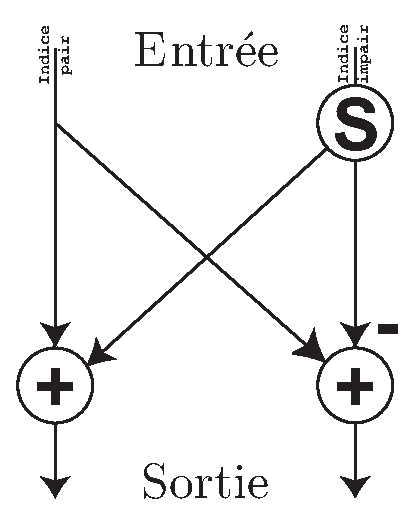
\includegraphics [scale = 0.7]{images/fft-butterfly-2points.eps}
    \end{center}
    \caption{Elementary butterfly diagram}
              \label{fig-fft-butterfly-2points}
\end{figure}
\begin{figure}[ht] 
    \begin{center}
    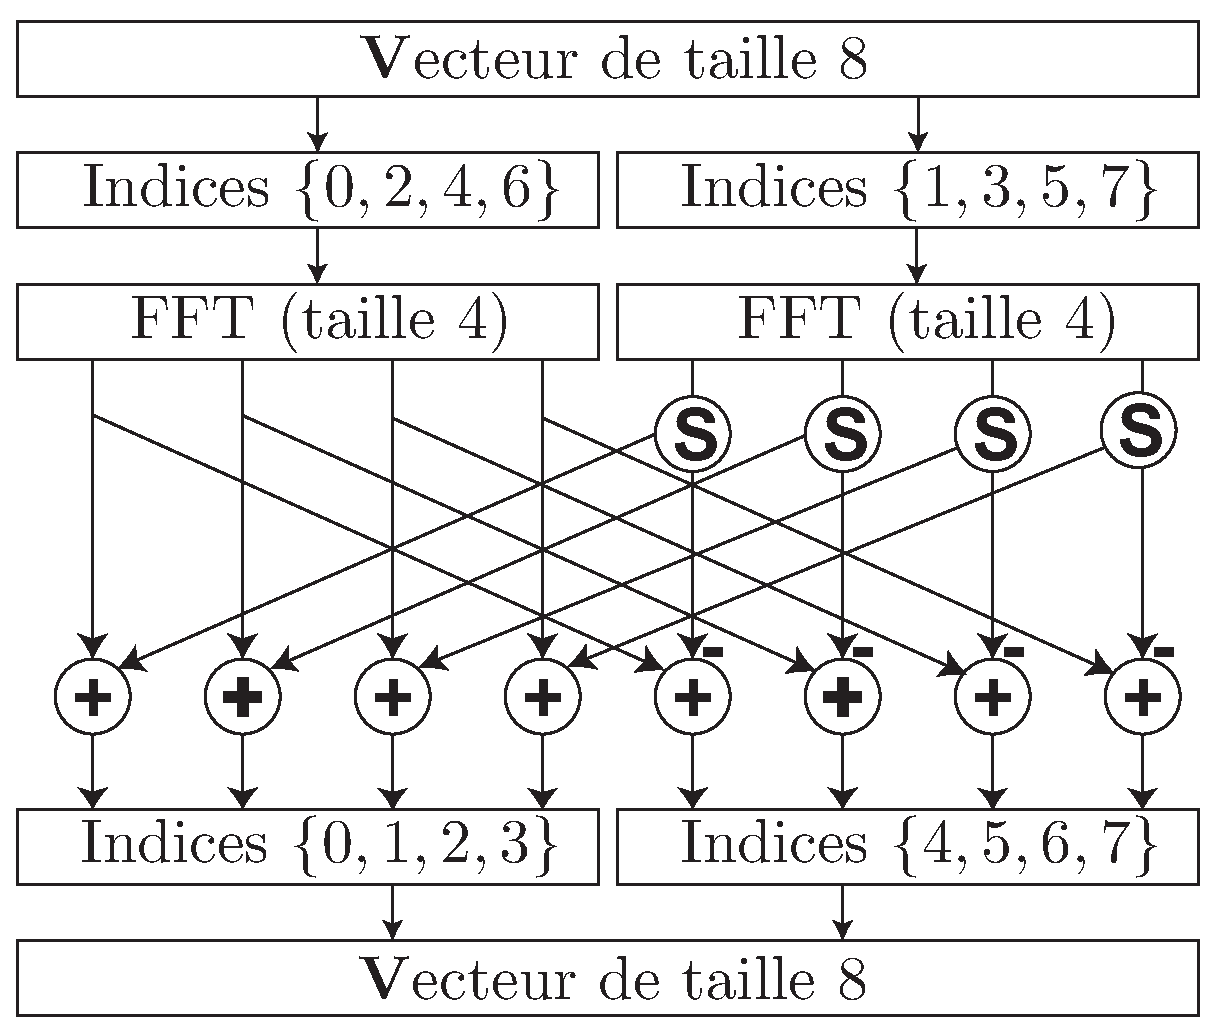
\includegraphics [scale = 0.5]{images/fft-butterfly-8points.eps}
    \end{center}
    \caption{An iteration of the FFT algorithm}
              \label{fig-fft-butterfly-8points}
\end{figure}
\end{rem}
 
 
 
\index{Algorithm!recursive} The simplest way to implement{\oe} the equations \eqref{eq-danielson-lanczos-a} and \eqref{eq-danielson-lanczos-b} is to use a recursive procedure. It is a known fact that a recursive procedure can be written, by means of loops, in a non-recursive fashion (but this process can sometimes be dangerous). We will see in the next paragraph \ref{sect2-impl-concrete} that the FFT algorithm has a lot to gain from being written non-recursively, and not only because of saving time. But for educational purposes, and in order to present some optimizations that can be done on the FFT implementation, we will focus on the recursive implementation written in the \ref{sect1-listing-fft} section.
 
 
The procedure \texttt{fft \_rec} therefore takes as input an integer \texttt{dir} which is worth $ + 1 $ or $ -1 $ depending on whether the Fourier transform is direct or inverse. To simplify the understanding of the code, a procedure \texttt{operator \_s} has been written to realize the operator $ \Ss^x_N $: it takes as input a vector as well as a real number $ x $ (which depends on the sign of the transform).
% ------------------------------------------------- -----
% ------------------------------------------------- -----
% sub-section - Cost analysis                            
% ------------------------------------------------- -----
% ------------------------------------------------- -----
\subsection{Cost analysis}
\label{sect2-analyze-cost-fft} 
 
Using the recurrence equations \eqref{eq-danielson-lanczos-a} and \eqref{eq-danielson-lanczos-b}, we easily calculate the cost of the algorithm.
 
\begin{prop}[Complexity of the FFT]
\index{Complexity} If we denote by $ C (N) $ the cost of the FFT algorithm for an input of length $N$, then $ C (N) $ satisfies the functional equation
\begin{equation*}
C (N) = 2 C (N / 2) + KN,
\end{equation*}
where $ K $ is some constant. In the end, we arrive at the expression $ C (N) = KN \log_2 (N) $.
\end{prop}
\begin{proof}
Computing $ \wh{f} $ requires computing $ \wh{f^1} $ and $ \wh{f^2} $ (i.e. $ 2 C (N / 2) $ operations), then mixing the two transforms by the butterfly diagram (i.e. $ KN $ operations). To reduce to a linear recurrence, it suffices to set $ P = \log_2 (N) $, and $ C'(N) = \frac{C (N)}{N} $ satisfies the functional equation $ C' (P) = C'(P-1) + K $. As $ C'(0) = 0 $, we deduce $ C' (P) = KP $, which allows us to conclude.
\end{proof}
The FFT algorithm may seem a bit magical, the fact remains that its discovery made it possible to make many calculations possible by reducing the cost of calculating $N$ Fourier coefficients by $ O(N^2) $ for a naive approach to $ O(N \log (N)) $. Its fairly recent discovery (in the mid-1960s) was a mini revolution: a calculation which until then required two weeks on a computer of the time was suddenly achievable in barely thirty seconds \footnote{Source: \cite{nr}, for $N$ of the order of $ 10^6 $}.
% ------------------------------------------------- -----
% ------------------------------------------------- -----
% sub-section - Variations around the algorithm                            
% ------------------------------------------------- -----
% ------------------------------------------------- -----
\subsection{Variations around the algorithm}
\label{sect2-variations-fft} 
 
Before describing a more efficient implementation of the FFT algorithm, let's make some additional remarks, which provide many variations around the proposed recursive implementation.
 
\begin{rem}{(\upshape \textbf{Length of entries}).} 
In the case where the length $N$ of the data of a sample $ \{f[n]\}_{n = 0}^{N-1} $ is not a power of two, we can make a calculation approximated by completing the sample with a sequence of zeros, to obtain a sample $ \{f_1 [n]\}_{n = 0}^{M-1} $, with $ M = 2^p $. Of course, we no longer calculate exactly the same transform, but in the case of an approximate calculation (calculation of continuous transforms, as explained in Section~\ref{sect1-link-trans-fourier-R}), this amounts to calculating the transform at slightly different frequencies, which is often acceptable.
\end{rem}
 
 
\begin{rem}{(\upshape \textbf{Calculation basis}).} 
\label{rmk-radix-fft}
\index{FFT!in base 4} The equations \eqref{eq-danielson-lanczos-a} and \eqref{eq-danielson-lanczos-b} which we used to implement the algorithm are the consequence of the sharing of vectors into two sub-vectors of size $ N / 2 $. This is called an FFT in \textit{base 2} (\textit{radix-2} in English). We can think of using another base, for example 4, which leads to considering sums of the four sub-FFTs of length $ N / 4 $. The advantage of such a choice (compared to base 2) is that one avoids making the obvious calculations of the fourth roots of the unit (which are coded simply by subtractions instead of additions in the formulas), which slightly reduces the number of operations to be performed. On the other hand, we must be careful, because the signs are not the same for the direct transform and for the reverse transform. To write the notations, we introduce the sub-vectors $ f^0 $, $ f^1 $, $ f^2 $ and $ f_3 $, of length $ N / 4 $, which are constructed from $ f $ in considering only the indices congruent respectively to 0, 1, 2 and 3 modulo 4. We also use $ \sigma $ which is worth $ + 1 $ for the direct transform, and $ -1 $ for the inverse transform. To discern the different portions of length $ N / 4 $ of the result, we will write $ \wh{f}^{(0/4)} $ for the first quarter, etc. Here are the equations:
\begin{align*}
\wh{f}^{(0/4)} & = \Ss_{N / 4}^{0/4} \wh{f^0} & + & \quad \Ss_{N / 4}^{1 / 4} \wh{f^1} & + & \quad \Ss_{N / 4}^{2/4} \wh{f^2} & + & \quad \Ss_{N / 4}^{3 / 4} \wh{f^3} \\
\wh{f}^{(1/4)} & = \Ss_{N / 4}^{0/4} \wh{f^0} & - & \quad \imath \sigma \Ss_{N / 4 }^{1/4} \wh{f^1} & - & \quad \Ss_{N / 4}^{2/4} \wh{f^2} & + & \quad \imath \sigma \Ss_{N / 4}^{3/4} \wh{f^3} \\
\wh{f}^{(2/4)} & = \Ss_{N / 4}^{0/4} \wh{f^0} & - & \quad \Ss_{N / 4}^{1 / 4} \wh{f^1} & + & \quad \Ss_{N / 4}^{2/4} \wh{f^2} & - & \quad \Ss_{N / 4}^{3 / 4} \wh{f^3} \\
\wh{f}^{(3/4)} & = \Ss_{N / 4}^{0/4} \wh{f^0} & + & \quad \imath \sigma \Ss_{N / 4 }^{1/4} \wh{f^1} & - & \quad \Ss_{N / 4}^{2/4} \wh{f^2} & - & \quad \imath \sigma \Ss_{N / 4}^{3/4} \wh{f^3}.
\end{align*}
By choosing an arbitrary basis $ p $, and by carrying out analogous calculations, one can handle vectors of size $ p^s $, which can be advantageous. Here is the recurrence formula in general:
\end{rem}
 
 
\begin{prop}
We keep the notations defined previously, but this time for the computation of a DFT using a $ p \geq 2 $ base. We have the equations
\begin{equation*}
\forall q = 0, \ldots, \, p-1, \quad \wh{f}^{(q / p)} = \sum_{k = 0}^{p-1}{e^{- \sigma \frac{2 \imath \pi}{p} kq} \cdot \Ss_{N / p}^{k / p} \wh{f^k}}.
\end{equation*}
\end{prop}
 
 
\begin{rem}
Of course, this formula is only interesting in practice when we know how to calculate explicitly and simply the factors $ e^{\frac{2 \imath \pi}{p} kq} $, for example for $ p = 2.4 , $ 8. The exercise \oldref{exo-algo-split-radix} shows how, by mixing both base 2 and base 4 transforms, we can further optimize the number of operations.
\end{rem}
 
% ------------------------------------------------- -----
% ------------------------------------------------- -----
% sub-section - The Cooley-Tukey transformation                            
% ------------------------------------------------- -----
% ------------------------------------------------- -----
\subsection{The Cooley-Tukey transformation}
\label{sect2-transfo-cooley-tukey} 
 
 
\index{Cooley-Tukey@\nompropreindex{Cooley-Tukey}} We have just seen an FFT algorithm which allows to very quickly calculate the Fourier transform of a vector whose size is $ 2^p $. But what if the size $N$ of the signal is not written in this form? The easy solution, if we just do approximate calculations, is to add zeros to reach a reasonable size, which will of course be the power of $ 2 $ immediately after $N$. But often, we cannot act as directly, and we have to find a finer algorithm, to take advantage of other properties of the integer $N$. This is how many other versions of the FFT algorithm have emerged since Cooley-Tukey's seminal article. In this chapter, different variants of the algorithm are presented, and some really allow us to get out of bad spots (for example the \textit{Good-Thomas} algorithm or the \textit{split-radix} algorithm, presented in the exercises \oldref{exo-algo-good-thomas} and \oldref{exo-algo-split-radix}).
 
 
In the case where the number $N$ is an integer that we know how to factorize, there is however a very simple method, which consists in looking more closely at the work carried out by the Cooley-Tukey method in the case where $ N = 2^s = 2 \times 2^{s-1} $. Thus, without $N$ necessarily being a power of 2, suppose that we have a factorization $ N = pq $. In the case where the integers $ p $ and $ q $ are coprime, a remarkable algebraic property (the Chinese lemma) makes it possible to optimize the calculations, and gives rise to the Good-Thomas algorithm already mentioned. But for now, let's not worry about such refinements, let's just follow step by step the transformations already done \guill{by hand} in paragraph \ref{sect2-present-algo-fft}. Recall the definition of the DFT of a vector $ f \in \CC^N $:
\begin{equation}
\label{eq-tfd-transfo-cooley-tukey}
\wh{f}[k] \eqdef \sum_{n = 0}^{N-1}{f[n] \omega_N^{- kn}} \quad \quad \text{for} \quad k = 0 , \ldots, \, N-1.
\end{equation}
The key idea to obtain a factorization of this expression is to perform a change of variables using the following two bijections:
\begin{equation*}
\begin{split}
\varphi: & \func{\{0, \ldots, \, q-1\} \times \{0, \ldots, \, p-1\}}{\{0, \ldots, \, N- 1\}}{(a, \, b)}{ap + b} \\
\psi: & \func{\{0, \ldots, \, p-1\} \times \{0, \ldots, \, q-1\}}{\{0, \ldots, \, N- 1\}}{(c, \, d)}{cq + d}.
\end{split}
\end{equation*}
We can indeed rewrite the sum \eqref{eq-tfd-transfo-cooley-tukey} in the form
\begin{equation*}
\begin{split}
\wh{f}[\psi (c, \, d)] & = \sum_{a = 0}^{q-1}{\sum_{b = 0}^{p-1}{\omega_N^{- (ap + b) (cq + d)} f[\varphi (a, b)]}} \\
& = \sum_{b = 0}^{p-1}{\omega_N^{- b (d + cq)} \sum_{a = 0}^{q-1}{\omega_q^{- ad} f[\varphi (a, b)]}}.
\end{split}
\end{equation*}
If we denote by $ f_b [a] \eqdef f[\varphi (a, \, b)] $ (which corresponds to taking only one column of $ f $, if we represent it in the form of a matrix of size $ p \times q $), then we get
\begin{equation}
\label{eqn-cooley-tukey-twiddle}
\wh{f}[\psi (c, \, d)] = \sum_{b = 0}^{p-1}{\omega_p^{- cb} \left(\omega_N^{- bd} \wh{f_b}[d] \right)}.
\end{equation}
\index{Twiddle factor} We have therefore succeeded in modifying the calculation algorithm to obtain an algorithm operating in 2D, on the size matrix $ p \times q $ that constitutes $ F \eqdef \{f[\varphi (a , b)]\}_{a, b} $. In fact, if we didn't have the parasitic terms $ \omega_N^{- bd} $ (often called \guill{twiddle factor} in English, see the exercise \oldref{exo-algo-split-radix}), we would simply be calculating the two-dimensional DFT of the 2D function $ F $ (which can also be considered as an image).
 
 
If we count the number of operations necessary to calculate the DFT of $ f $ by this method, we obtain $ C pq (p + q) $, where $ C $ represents a constant taking into account the calculation time of complex additions and multiplications. But the advantage of the method is that it can be applied recursively to each of the sub-DFTs to be calculated. Thus, if $N$ is factored in the form $ p_1 \times p_2 \times \cdots \times p_s $, we obtain a number of operations proportional to $ N \sum{p_i} $. Of course, in the case where $ N = 2^s $, we find the traditional FFT algorithm already described in paragraph \ref{sect2-present-algo-fft}. However, we see that with a little adaptation, we can easily take into account $N$ admitting more complex decompositions. Be careful, however, not to fall into an excess of optimism: this method will be totally inefficient when $N$ is factored badly. In this case, we must opt for other approaches, such as the one suggested in the \oldref{exo-chirp-transform-finis-corps} exercise. Moreover, when the factorization $ N = pq $ has particularities (typically if $ p $ and $ q $ are coprime), there are more optimized algorithms, like that of \textit{Good-Thomas} presented at l'exercise \oldref{exo-algo-good-thomas}.
% ------------------------------------------------- -----
% ------------------------------------------------- -----
% sub-section - Concrete implementation                            
% ------------------------------------------------- -----
% ------------------------------------------------- -----
\subsection{Concrete implementation}
\label{sect2-impl-concrete} 
 
 
The naive implementation presented in paragraph \ref{sect2-present-algo-fft} (in the case $ N = 2^p $) suffers from many weak points, among which we can note: \begin{rs}
\item \textit{a recursive structure}: Recursive calls require additional system instructions, which wastes a lot of time.
\item \textit{a use of temporary memories}: the explicit computation of the two subvectors $ f^0 $ and $ f^1 $ of size $ N / 2 $ is obviously an enormous loss of memory (since redundant information is created).
\end{rs} We will see in this paragraph how to implement a routine that solves these two problems at once. The main idea is to rearrange the starting vector. We want the elements of the vector to be arranged so that at each subdivision (in the form of two vectors of half size), the first vector is the $ N / 2 $ first entries, and the second vector is the $ N / 2 $ last (and not the even and odd indices). For an implementation in a classic language (C or C ++ for example), the gain will be enormous: by the use of pointers (or, for the uninitiated, by moving the start of the array), the only memory used by the vector of origin allows to accommodate the two sub-tables.
 
 
In the following, we will note the indices in binary form, that is to say
\begin{equation*}
i = [i_{p-1} \ldots i_0]_b = \sum_{t = 0}^{p-1}{i_t 2^t}.
\end{equation*}
Our goal is to start the algorithm with a vector $ g \eqdef \{f[n_p (0)], \ldots, \, f[n_p (N-1)]\} $, where $ i \mapsto n_p ( i) $ denotes a permutation of the indices. We want that when applying the equation of \textit{Danielson-Lanczos}
\begin{equation}
\label{eq-rec-relation-fft}
\wh{g}[k] = \wh{g^0}[k] + \omega_N^{- k} \wh{g^1}[k],
\end{equation}
the vector $ g^0 $ is made up of the entries of $ f $ with indices $ 0, \ldots, \, N / 2-1 $, and that the vector $ g^1 $ is made up of the entries of $ f $ d'indices $ N / 2, \, \ldots, \, N-1 $. Thus, dividing $ g $ in two is done without having to move values in the memory of the computer. So that this construction still works during recursive calls on $ g^0 $ and $ g^1 $, these two subvectors are themselves permuted from $ f^0 $ and $ f^1 $ by $ n_{p- 1} $, which meets the same requirements as $ n_p $. This condition, translated on the permutation $ n_p $, is expressed as follows:
\begin{equation*}
n_p ([i_{p-1} \ldots i_0]_b) = i_0 2^{p-1} + n_{p-1} ([i_{p-1} \ldots i_1]_b).
\end{equation*}
By iterating this equation $ p $ times, we find the expression for the permutation $ n_p $:
\begin{equation*}
n_p (i) = n_p ([i_{p-1} \ldots i_0]_b) = \sum_{t = 0}^{p-1}{i_t 2^{p-1-t}}.
\end{equation*}
More concisely, $ n_p (i) $ is the transpose of $ i $ written in binary. For example, for $ N = 8 $, if $ i = 6 $, which is written $ 110 $ in binary, then $ n_p (i) $ will be written $ 011 $, i.e. $ n_p ( 6) = $ 3.
 
 
In the end, we see that we must classify the elements of the vector according to the reverse binary writing of the indices. This is what the \texttt{rev \_bits} procedure, described in \listingterme{} \ref{listing-rev_bits}, does. This procedure requires $ O(N) $ operations. For a more refined implementation, we can look at the \nompropre{Numerical Recipes} \cite{nr}. Figure \figref{fig-rev-bit-matrix} shows the permutation matrix corresponding to $ n_p $, i.e. the matrix $ M^{(p)} $ such that $ M_{ij}^{(p)} = \delta_{i}^{n_p (j)} $. The black dots represent the non-zero entries (equal to $ 1 $) in the matrix $ M^{(p)} $. \begin{figure}[ht]
    \begin{center}
    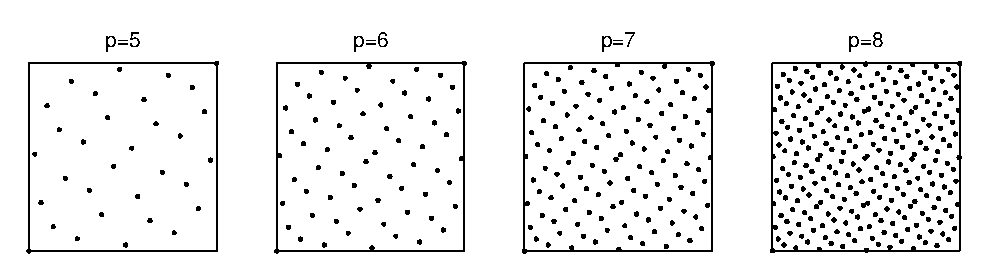
\includegraphics [scale = 0.6]{images/rev-bit-matrix.eps}
    \end{center}
    \caption{Bit inversion matrix}
              \label{fig-rev-bit-matrix}
\end{figure}
The exercise \oldref{exo-bit-reversal} proposes to write a recursive function to perform the bit reversal. Using the \texttt{rev \_bits} procedure allows you to write a \texttt{fft \_dit} function that does not use temporary memory. The end of this procedure replaces the recursive calls with nested \texttt{\pfor} loops. The figure \figref{fig-inversion-bits} shows the operations to perform to reverse the inputs of a vector, highlighting the necessary permutations. \begin{figure}[ht]
    \begin{center}
    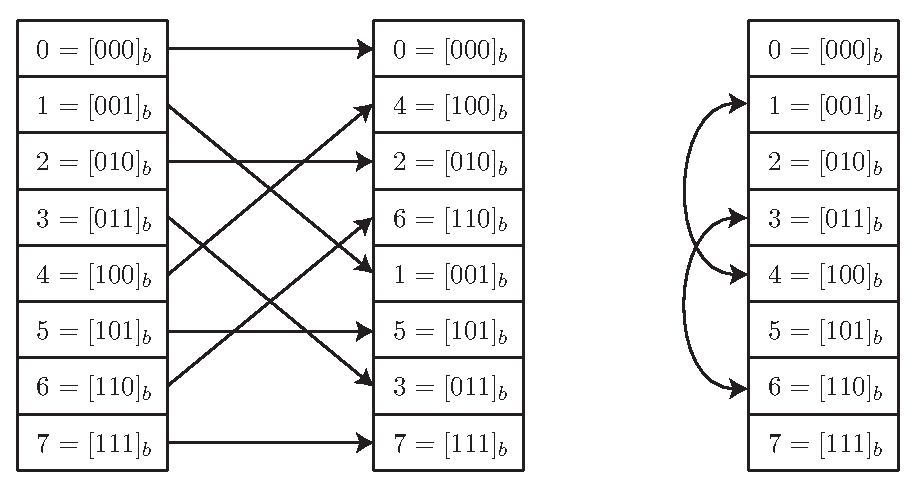
\includegraphics [scale = 0.6]{images/inversion-bits.eps}
    \end{center}
    \caption{Inversion of bits by permutation of inputs}
              \label{fig-inversion-bits}
\end{figure}
 
% ------------------------------------------------- -----
% ------------------------------------------------- -----
% sub-section - Frequency decimation                            
% ------------------------------------------------- -----
% ------------------------------------------------- -----
\subsection{Frequency decimation}
\label{sect2-frequency-decimation} 
 
 
\index{Frequency!decimation} We are going to redo the calculations that led to the equations \eqref{eq-danielson-lanczos-a} and \eqref{eq-danielson-lanczos-b}, but this time by performing a grouping according to the frequencies of the transform. The algorithm that we will obtain will be in a way the symmetric of the \guill{classical} algorithm proposed by \nompropre{Cooley} and \nompropre{Tukey}. Even if this new implementation will not improve speed of execution, it is important to have in mind the two dual versions of the FFT, just as it is important to master the temporal and frequency properties of the Fourier transform.
 
 
In accordance with the notations \eqref{eq-part-gd}, we denote by $ f_g $ (resp. $ F_d $) the $ N / 2 $ first entries (resp. $ N / 2 $ last) of the vector $ f $. We have
\begin{equation*}
\wh{f}[k] = \sum_{n = 0}^{N / 2-1}{\left(f_g [n] + e^{- k N / 2 \frac{2 \imath \pi}{N}} f_d [n] \right) e^{- nk \frac{2 \imath \pi}{N}}}.
\end{equation*}
We are therefore led to make a distinction according to the parity of $ k $. By following the notations of the equation \eqref{eq-part-even-odd}, we consider $ (\wh{f} \:)^0 $ (resp. $ (\wh{f} \:)^1 $) the even (resp. odd) part of the transformed vector. Be careful, these vectors should not be confused with $ \wh{f^0} $ and $ \wh{f^1} $, which are the transforms of the vectors $ f^0 $ and $ f^1 $. We therefore write, for $ k \in \{0, \ldots, \, N / 2-1\} $,
\begin{align*}
(\wh{f} \:)^0 [k] & = \wh{f}[2k] = \sum_{n = 0}^{N / 2-1}{\left(f_g [n] + f_d [n] \right) e^{- nk \frac{2 \imath \pi}{N / 2}}} \\
(\wh{f} \:)^1 [k] & = \wh{f}[2k + 1] = \sum_{n = 0}^{N / 2-1}{e^{- k \frac{2 \imath \pi}{N}} \left(f_g [n] - f_d [n] \right) e^{- nk \frac{2 \imath \pi}{N / 2}}}.
\end{align*}
By using the operator $ \Ss_N^x $ introduced in \eqref{eq-operator-S}, we obtain the following recurrence equations:
\begin{align*}
(\wh{f} \:)^0 & = \Ff \left(f_g + f_d \right) \\
(\wh{f} \:)^1 & = \Ff \left(\Ss_{N / 2}^{1/2} (f_g - f_d) \right).
\end{align*}
 
 
 
Contrary to the technique of temporal decimation, we see that the sub-vectors for which we must calculate the Fourier transform are directly obtained from the input vector (just take the left and right parts). On the other hand, the output vector must be composed, according to the parity of the index, either of the values of one transform or of the other. To avoid having to use temporary memory, we will use the same trick as for the temporal decimation, but in the other direction. We will be satisfied with juxtaposing the two transforms, that is to say putting the vectors $ (\wh{f} \:)^0 $ then $ (\wh{f} \:)^1 $. To obtain the correct result, it will suffice, at the end of the procedure, to put the frequencies back in the correct order, by calling the \texttt{rev \_bits} function. We can then write a non-iterative version of the FFT which uses the principle of frequency decimation, it is the procedure \texttt{fft \_dif} which is written in paragraph \ref{listing-fft_dif}.
 
\begin{rem}{(\upshape \textbf{Time and frequency}).} 
We can see that the frequency decimation is exactly symmetrical to the temporal decimation. Acting on the indices of the result vector (i.e. on the frequencies) instead of acting on the indices of the input vector results in a reversal of the bits in the final phase of the algorithm .
\end{rem}
 
 
 
To conclude, we can already notice the wide variety of variations of the FFT algorithm at our disposal. Many other methods will also be described in the following chapters and exercises. The literature revolving around FFT is gigantic, it is undoubtedly one of the most extensive fields of numerical analysis. Review articles have been written, for example by \nompropre{Burrus} \cite{burrus-fft}. The question is therefore to know which is the best method. Of course, there is no definitive answer, because too many factors come into play, not only concerning the length of the transform and the type of data (real, complex, etc.), but above all the type of architecture (machine, operating system, parallel architecture, memory cache, etc.) and the type of precision desired. If in doubt, it is better to stay on a simple, but robust implementation, even if it means sacrificing a little efficiency.
% ------------------------------------------------- -----
% ------------------------------------------------- -----
% sub-section - Matrix writing                            
% ------------------------------------------------- -----
% ------------------------------------------------- -----
\subsection{Matrix writing}
\label{sect1-matrix-writing} 
 
 
\index{Vandermonde!matrix} \index{Unit!matrix} \index{Unitary!endomorphism} \index{Interpolation} If we write the matrix $ \Omega_N $ of the linear operator $ \Ff: \CC^N \rightarrow \CC^N $ in canonical bases, we get
\begin{equation}
\label{eq-defn-matrix-fourier}
\Omega_N \eqdef \begin{pmatrix} 1 & 1 & 1 & \ldots & 1 \\1 & \omega_N^{-1} & \omega_N^{- 2} & \ldots & \omega_N^{- (N- 1)} \\1 & \omega_N^{- 2} & \omega_N^{- 4} & \ldots & \omega_N^{- 2 (N-1)} \\\vdots & \vdots & \vdots & \vdots & \vdots \\1 & \omega_N^{- (N-1)} & \omega_N^{- 2 (N-1)} & \ldots & \omega_N^{- (N-1) (N-1 )} \end{pmatrix}.
\end{equation}
This matrix corresponds to a matrix of \textit{Vandermonde}. These matrices occur when we write the linear system corresponding to the search for the unique polynomial of degree $N$ passing through $N$ distinct points. There is nothing surprising about this, since we will see in Section~\ref{sect1-calculations-products}, that the computation of inverse DFT corresponds to the computation of the coefficients of the interpolation polynomial at points quite particular, the \ordin{N}{th} roots of the unit.
 
 
\label{notation-47} The formula of the inverse Fourier transform \eqref{eq-transforme-fourier-discr-inverse} results in the fact that the inverse of the matrix $ \Omega_N $ is the matrix $ \frac{1}{N} \Omega_N^* $, where we denote by $ M^* \eqdef \transp{\ol{M}} $ the adjoining matrix of $ M $. This means that the matrix $ \frac{1}{\sqrt{N}} \Omega_N $ is unitary, that is to say $ \Omega_N \Omega_N^* = N \Id_N $. The equations of \textit{Danielson-Lanczos} \eqref{eq-danielson-lanczos-a} and \eqref{eq-danielson-lanczos-b} can then be written in the form of a factorization of the matrix $ \Omega_N $:
\begin{equation*}
\Omega_N \begin{pmatrix} a_0 \\\vdots \\a_{N-1} \end{pmatrix} = \begin{pmatrix} \Omega_{N / 2} & \Delta_{N / 2} \Omega_{N / 2} \\\Omega_{N / 2} & - \Delta_{N / 2} \Omega_{N / 2} \end{pmatrix} \begin{pmatrix} a_0 \\\vdots \\a_{N-2 } \\a_1 \\\vdots \\a_{N-1} \end{pmatrix},
\end{equation*}
where we noted $ \Delta_{N / 2} = \diag (1, \, \omega_N^{-1}, \ldots, \, \omega_N^{- (N / 2-1)}) $.

% ------------------------------------------------- -----
% ------------------------------------------------- -----
% ------------------------------------------------- -----
% section - Circular convolution                            
% ------------------------------------------------- -----
% ------------------------------------------------- -----
% ------------------------------------------------- -----
\section{Circular convolution}
% \addcontentsline{toc}{section}{Circular convolution}
\label{sect1-tfd-prod-convol} 
 
\index{Convolution!circular} \index{Group!cyclic} We have defined in paragraph \ref{sect2-convolution-transforme-fourier}, the product of convolution on any abelian group, and we will now apply this definition as well as the convolution theorem \ref{thm-convolution-trans-fourier-grpe-abelien}, in the simple case of a cyclic group, and more precisely by using the language of the discrete Fourier transform which was defined in paragraph \ref{sect1-language-processing-signal}.
% ------------------------------------------------- -----
% ------------------------------------------------- -----
% sub-section - Circular convolution                            
% ------------------------------------------------- -----
% ------------------------------------------------- -----
\subsection{Circular convolution}
\label{sect1-convolution-circular} 
 
\index{Convolution!circular} Let us start by recalling the definition of the convolution product as well as the main results already obtained.
 
\begin{defn}[Discrete convolution product]
\index{Convolution product!discrete} Let $ \{f[n]\}_{n = 0}^{N-1} $ and $ \{g [n]\}_{n = 0}^{N-1} $ two discrete samples (assumed to represent signals sampled at the same times, regularly spaced). We define the convolution product $ f * g $ of the two signals by the equation
\begin{equation}
\label{eq-convolution-discrete}
(f * g) [n] \eqdef \sum_{k = 0}^{N-1}{f[k] g [nk]}, \quad \quad n = 0, \ldots, \, N-1 .
\end{equation}
\end{defn}
 
 
\begin{rem}
In the equation \eqref{eq-convolution-discrete}, the quantity $ nk $ is of course calculated modulo $N$, which amounts to considering the samples $ f $ and $ g $ as periodic functions of period $N$. This formula is the translation of the equation \eqref{eq-formula-prod-convol-grpe-abelien}, in the case of the group $ G = \ZZ/N \ZZ $, taking care to use an additive notation instead of multiplicative notation. From the perspective of a computer implementation, we can give a more explicit formula:
\begin{equation*}
(f * g) [n] \eqdef \sum_{k = 0}^{n}{f[k] g [nk]} + \sum_{k = n + 1}^{N-1}{f[ k] g [n-k + N]}, \quad \quad n = 0, \ldots, \, N-1.
\end{equation*}
\end{rem}
 
 
\begin{prop}
The circular convolution product is commutative, and the mapping $ (f, \, g) \mapsto f * g $ endows $ \CC^N $ with an algebra structure.
\end{prop}
\begin{proof}
The only non-trivial thing to check is the commutativity, which is obtained by making the change of variable $ k'= nk $ in the equation \eqref{eq-convolution-discrete}.
\end{proof}
We can now state the convolution theorem \ref{thm-convolution-trans-fourier-grpe-abelien}, in terms of a discrete Fourier transform.
 
\begin{prop}[Convolution and TFD]
\label{prop-convol-tfd}
Let $ \{f[n]\}_{n = 0}^{N-1} $ and $ \{g [n]\}_{n = 0}^{N-1} $ two discrete samples. We have the convolution formula
\begin{equation}
\label{eq-formula-convolution-tfd}
\forall n \in \{0, \ldots, \, N-1\}, \quad \wh{f * g}[n] = \wh{f}[n] \wh{g}[n].
\end{equation}
\end{prop}
\begin{proofnoqed}
For the explanations to be clearer, we will write $ f_1 $ and $ g_1 $ the functions of $ \ZZ/N \ZZ $ in $ \CC $ associated with the samples $ f $ and $ g $ (which are of size $N$). We then have, for $ n \in \{0, \ldots, \, N-1\} $ (where, in terms of an abelian group, $ n \in \ZZ/N \ZZ $),
\begin{equation}
\label{eq-lien-tfd-trans-fourier}
\wh{f}[n] = \wh{f_1} (\chi_n) \quad \quad \text{et} \quad \quad \wh{g}[n] = \wh{g_1} (\chi_n),
\end{equation}
where we noted $ \{\chi_0, \ldots, \, \chi_{N-1}\} $ the characters, that is to say the elements of the dual $ \wh{\ZZ/N \ZZ} $ (see the equation \eqref{eq-formula-character-znz}). Using the theorem \ref{thm-convolution-trans-fourier-grpe-abelien}, for the functions $ f_1 $ and $ g_1 $ on $ G = \ZZ/N \ZZ $, we obtain
\begin{equation*}
\wh{f_1 * g_1} (\chi_n) = \wh{f_1} (\chi_n) \wh{g_1} (\chi_n).
\end{equation*}
However, we also have
\begin{equation*}
\wh{f * g}[n] = \wh{f_1 * g_1} (\chi_n).
\end{equation*}
This thus makes it possible to write, using the equations \eqref{eq-lien-tfd-trans-fourier},
\begin{equation*}
\wh{f * g}[n] = \wh{f_1} (\chi_n) \wh{g_1} (\chi_n) = \wh{f}[n] \wh{g}[n]. \tag *{\qed}
\end{equation*}
\end{proofnoqed}
 
 
\begin{rem}{(\upshape \textbf{Finite signals and periodization}).} 
\index{Periodization} The main theoretical difficulty of the discrete Fourier transform is the assimilation between our sample $ \{f[n]\}_{n = 0}^{N-1} $ and a function $ f $ set to $ \ZZ/N \ZZ $. This assimilation has the advantage of obtaining algebraic formulas at a lower cost such as the result of inversion \ref{prop-tfd-inverse} as well as that of convolution \ref{prop-convol-tfd}. However, this approach implies that our function $ f $, if we look at it as a signal in time is in fact a periodic function, of period $N$. This goes against the natural intuition which wants us to consider our (finite) signal $ f $ as zero outside the interval in which it is defined. It is on this point that we will have to pay attention when we want to calculate the convolution products between two finite signals. It is precisely this problem which is raised in Paragraph~\ref{sect1-convolution-acyclic} during the study of non-circular convolution.
\end{rem}
 
% ------------------------------------------------- -----
% ------------------------------------------------- -----
% sub-section - Calculation with the FFT                            
% ------------------------------------------------- -----
% ------------------------------------------------- -----
\subsection{Calculation with the FFT}
\label{sect1-convolution-calcul-fft} 
 
A naive implementation of the equation \eqref{eq-convolution-discrete} leads to a number of operations (complex multiplications and additions) of the order of $ O(n^2) $. Indeed, it is necessary to calculate the $N$ values of the convolée, and each time, a sum of $N$ products appears. However, using the convolution formula \eqref{eq-formula-convolution-tfd} and the inversion formula \eqref{eq-transforme-fourier-discr-inverse}, we can write an equation that will turn out to be very useful :
\begin{equation*}
f * g = \Ff^{-1} \left(\wh{f} \cdot \wh{g} \right),
\end{equation*}
where we noted $ f $ and $ g \in \CC^N $ two samples of size $N$. Thanks to the FFT algorithm, the calculation of the transforms $ \wh{f} $ and $ \wh{g} $ can be done in a number of operations of the order of $ O(N \log (N) ) $, and the computation of the product $ \wh{f} \cdot \wh{g} $ requires of course only $N$ complex multiplications. In the end, we thus manage to calculate a convolution product with a number of operations of the order of $ O(N \log (N))$.

% ------------------------------------------------- -----
% ------------------------------------------------- -----
% sub-section - Acyclic convolution                            
% ------------------------------------------------- -----
% ------------------------------------------------- -----
\subsection{Acyclic convolution}
\label{sect1-convolution-acyclic} 
 
 
\index{Convolution!acyclic} We are going to leave for a short time the transformations linked to the group structure of $ \ZZ/N \ZZ $ to define an operation which does not respect this cyclic structure at all, the acyclic convolution (also called linear convolution), denoted $ \star $ (not to be confused with the $ * $ of cyclic convolution). The support of a $ f \in \CC^\ZZ $ signal is defined by
\begin{equation*}
\Supp (f) \eqdef \enscond{n \in \ZZ}{f[n] \neq 0}.
\end{equation*}
We start by defining the acyclic convolution for two signals $ \{f_1 [n]\}_{n \in \ZZ} $ as well as $ \{f_2 [n]\}_{n \in \ZZ} $ whose support is assumed to be finite, which means that $ \Supp (f_1) $ and $ \Supp (f_2) $ are finite sets. We then define the sequence $ f_1 \star f_2 $ by
\begin{equation}
\label{eq-convolution-acyclic}
\forall n \in \ZZ, \quad f_1 \star f_2 [n] = \sum_{k \in \ZZ}{f_1 [k] f_2 [nk]}.
\end{equation}
Note that we have the very useful equation:
\begin{equation*}
\Supp (f_1 \star f_2) \subset \Supp (f_1) + \Supp (f_2) \eqdef \enscond{n + p}{n \in \Supp (f_1), \; p \in \Supp (f_2)}.
\end{equation*}
Linear convolution therefore has nothing to do with cyclic convolution, which is an operation on vectors of $ \CC^N $ (and results in a vector of $ \CC^N $). However, by creating from our two sequences, two vectors $ \wt{f_1} $ and $ \wt{f_2} $ of size $N$ sufficiently large, we will see that we can calculate the non-zero values of $ f_1 \star f_2 $ as some entries of the vector $ \wt{f_1} * \wt{f_2} $.
 
 
\index{Support} Let us start by noticing that the size necessary to store the entries of $ f_1 \star f_2 $ is $ N \eqdef N_1 + N_2 - 1 $, where we have noted $ N_1 $ and $ N_2 $ the sizes supports of $ f_1 $ and $ f_2 $. We can translate the indices of $ f_1 $, which allows us to assume that they are $ \{0, \ldots, \, N_1-1\} $. This implies that we must perform the same translation on the vector $ f $. So let's start by creating a vector $ \wt{f_1} \in \CC^{N} $ by first copying the non-zero $ N_1 $ entries of $ f_1 $, then adding zeros. The construction of the vector $ \wt{f_2} $ is a little more difficult, since it is necessary to take into account the negative indices. Copy the entries with positive indices of $ f_1 $ into $ \wt{f_2} \in \CC^{N} $, then put enough zeros, then copy the entries with negative indices. More precisely, if we write $ \Supp (f_2) = \{- P, \ldots, \, 0, \ldots, \, Q\} $, with $ N_2 = Q + P + 1 $, then we will have
\begin{equation*}
\wt{f_2} \eqdef \{f_2 [0], \, f_2 [1], \ldots, \, f_2 [Q], \, 0, \ldots, \, 0, \, f_2 [-P], \ldots, \, f_2 [-1]\} \in \CC^N.
\end{equation*}
Once all these transformations have been carried out, we can finally write:
\begin{equation*}
\forall n \in \{0, \ldots, \, N_1 + Q-1\}, \quad f_1 \star f_2 [n] = \wt{f_1} * \wt{f_2}[n].
\end{equation*}
For indices located in the interval $ \{- P, \ldots, \, -1\} $, care must be taken because, due to circular convolution, they have been moved in the interval $ \{NP , \ldots, \, N-1\} $. However, in practice (for example, for filtering), we only use the indices $ \{0, \ldots, \, N_1\} $.
 
 
Once this transformation is done, we can of course use the algorithm presented in Section~\ref{sect1-convolution-calcul-fft} to quickly calculate the convolution. This algorithm, which goes hand in hand with the technique of adding zeros that we have just explained, will allow filtering to be carried out quickly. All this will be explained in detail in paragraph \ref{sect1-filtering}. It may be noted that when the size of one of the two vectors is much smaller than that of the other, there is a strategy which makes it possible to avoid adding too many zeros at the end of the shorter vector. This method is exposed to the exercise \oldref{exo-calcul-convolution-fft}.
 
 
In the following, we will often directly consider the linear convolution of two vectors of $ \CC^N $, and in this case, the negative indices will be placed at the end of the vector, (it will therefore be necessary to add zeros between the positive indices and these negative indices to be able to use the FFT algorithm). However, it must be remembered that cyclic and acyclic convolutions give very different results. For example, the figure \figref{fig-diff-conv-linear-circular} shows a comparison of the two convolutions. Filtering by $ g $ performs a kind of \guill{local mean}. For the central values of $ k $, more precisely $ 2 \leq k \leq N-4 $, we have $ f * g [k] = f \star g [k] $. However, for the edge values, we find different results. \begin{figure}[ht]
    \begin{center}
    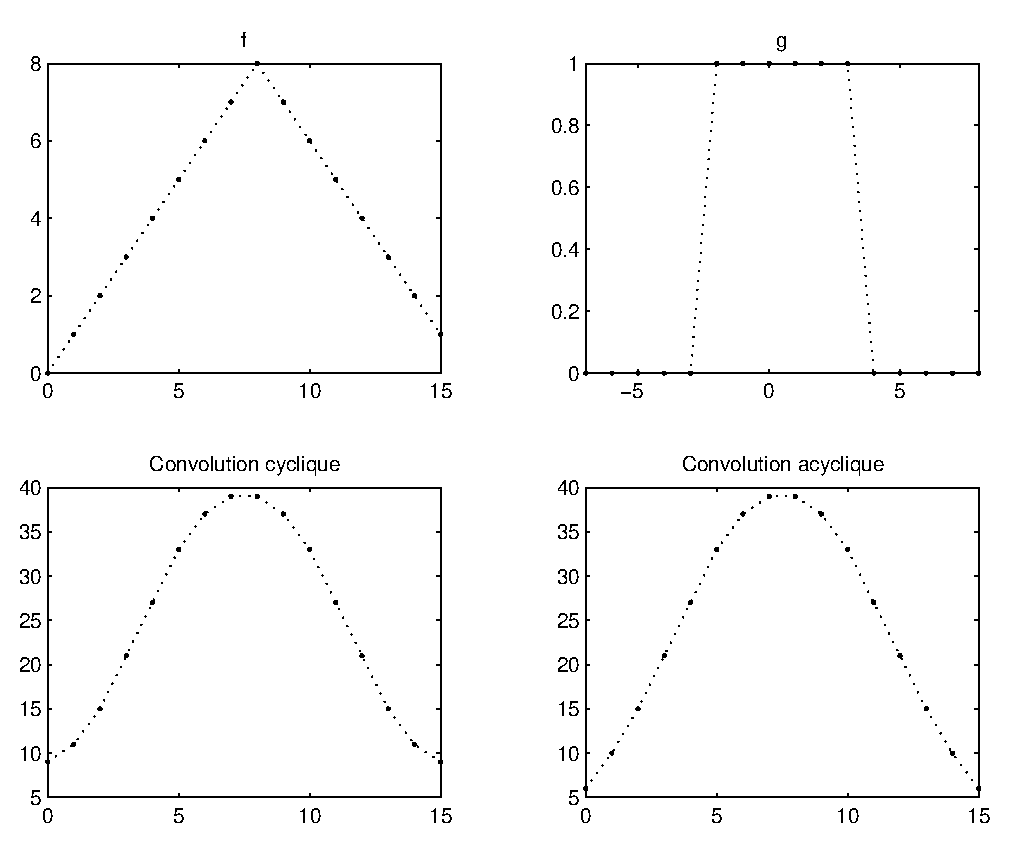
\includegraphics [scale = 0.6]{images/diff-conv-lineaire-circulaire.eps}
    \end{center}
    \caption{Cyclic and acyclic convolutions}
              \label{fig-diff-conv-linear-circular}
\end{figure}
Thus, in the majority of applications where the vector $ x $ will represent a temporal signal, acyclic convolution will be preferred, so as not to alter the values on the edges. All this will be covered in detail when explaining the different types of filtering, in Section~\ref{sect1-filtering}.

% ------------------------------------------------- -----
% ------------------------------------------------- -----
% ------------------------------------------------- -----
% section - In higher dimension                            
% ------------------------------------------------- -----
% ------------------------------------------------- -----
% ------------------------------------------------- -----
\section{In higher dimension}
% \addcontentsline{toc}{section}{In higher dimension}
\label{sect1-tfd-dim-sup} 
 
 
In this paragraph, to simplify the explanations, we will restrict ourselves to calculations of transforms in dimension 2. Generalization to higher dimensions, even if it can be dangerous from the point of view of programming, does not present theoretical difficulties.
% ------------------------------------------------- -----
% ------------------------------------------------- -----
% sub-section - Discrete Fourier transform in 2D                            
% ------------------------------------------------- -----
% ------------------------------------------------- -----
\subsection{Discrete Fourier transform in 2D}
\label{sect2-transforme-discrete-2d} 
 
\index{Fourier transform!in 2D}
 
\begin{defn}[two-dimensional DFT]
A two-dimensional sample is represented by a matrix $ \left\{f[i, \, j] \right\} \in \CC^{N \times P} $. \\The indices are therefore $ i \in \{0, \ldots, \, N-1\} $ and $ j \in \{0, \ldots, \, P-1\} $. Its discrete Fourier transform is a $ N \times P $ matrix defined by
\begin{equation}
\label{eq-defn-tfd-2d}
\wh{f}[k, \, l] \eqdef \sum_{i, \, j}{f[i, \, j] e^{- \frac{2 \imath \pi}{N} ik} e^{- \frac{2 \imath \pi}{P} jl}},
\end{equation}
where $ k \in \{0, \ldots, \, N-1\} $ and $ l \in \{0, \ldots, \, P-1\} $.
\end{defn}
As for the one-dimensional case, we can still make the link with the Fourier transform on an abelian group, by considering the group $ G \eqdef \ZZ/N \ZZ \times \ZZ/P \ZZ $. The characters in this group are $ \chi_{ij} $, for $ 0 \leq i <N $ and $ 0 \leq j <P $, defined by
\begin{equation*}
\forall (n, p) \in \ZZ/N \ZZ \times \ZZ/P \ZZ, \quad \chi_{ij} (n, p) \eqdef \left(\omega_N \right)^{- in } \left(\omega_P \right)^{- jp}.
\end{equation*}
We can therefore translate the equation \eqref{eq-defn-tfd-2d} by
\begin{equation*}
\forall k \in \{0, \ldots, \, N-1\}, \; \forall l \in \{0, \ldots, \, P-1\}, \quad \wh{f}[k, \, l] = \wh{f} (\chi_{kl}),
\end{equation*}
where we noted $ f $ both the sample and the associated function $ f: G \rightarrow \CC $.
 
\index{Isomorphism} Once again, we see that the function
\begin{equation*}
\Ff: \func{\CC^{N \times P}}{\CC^{N \times P}}{f}{\Ff(f) = \wh{f}}
\end{equation*}
is an algebra isomorphism of which we explicitly know the reverse.
 
\begin{prop}[2D inversion formula]
Let $ f \in \CC^{N \times P} $ be a 2D sample of size $ N \times P $. We have the inversion formula
\begin{equation*}
f[i, \, j] = \frac{1}{NP} \sum_{k, \, l}{\wh{f}[k, \, l] e^{\frac{2 \imath \pi }{N} ik} e^{\frac{2 \imath \pi}{P} jl}},
\end{equation*}
for $ i \in \{0, \ldots, \, N-1\} $ and $ j \in \{0, \ldots, \, P-1\} $.
\end{prop}
 
 
 
The important point is of course whether we still have a fast algorithm to calculate the DFT in dimension two. The answer is given by a simple rewrite of the equation \eqref{eq-defn-tfd-2d}, for $ k \in \{0, \ldots, \, N-1\} $ and $ l \in \{0, \ldots, \, P-1\} $:
\begin{equation*}
\wh{f}[k, \, l] = \sum_{i = 0}^{N-1}{\left(\sum_{j = 0}^{P-1}{f[i, \, j] e^{- \frac{2 \imath \pi}{P} jl}} \right) e^{- \frac{2 \imath \pi}{N} ik}} = \sum_{i = 0 }^{N-1}{\wh{F_i}[l] e^{- \frac{2 \imath \pi}{N} ik}},
\end{equation*}
where we denote by $ F_i \in \CC^P $ the vector formed by the \ordin{i}{ith} row of the matrix $ f $, and $ \wh{F_i} $ its one-dimensional DFT.
 
 
To calculate the TFD in 2D of a $ f $ matrix, it is therefore sufficient to calculate the TFD of each of its rows, then to calculate the TFD of the columns of the matrix obtained. In a more synthetic way, we can write matricially:
\begin{equation*}
\wh{f} = \transp{\Ff_{\text{1D}} \left(\transp{\Ff_{\text{1D}} (f)} \right)},
\end{equation*}
where the operator $ \Ff_{\text{1D}} $ performs the one-dimensional DFT on the rows of a matrix. It is also possible to carry out the calculations in the reverse direction, that is to say first calculate the transform on the columns, then on the rows. Matrix, like $ \transp{\Omega_N} = \Omega_N $, the transformation equation is written $ \wh{f} = \Omega_N f \Omega_P $, where $ \Omega_N $ is defined at the equation \eqref{eq-defn-matrix-fourier}.
 
 
\index{Oscillation} Figure \figref{fig-tfd-2d} shows the 2D Fourier transform of an image, which is just another way of representing a 2D sample (the values of the function are represented by levels gray, varying from black for 0 to white for 1). We can intuitively interpret the spectrum obtained. The value of $ \wh{f}[i, \, j] $, which we can \guill{read} directly on the image representing the spectrum, corresponds to a certain amount of(two-dimensional) oscillations present in the image. Please note, for the Fourier transform (right image), the large coefficients are shown in black. These oscillations are characterized by a frequency, $ \frac{1}{N} \sqrt{i^2 + j^2} $, and a direction, that of the vector $ (i, \, j) $. 
	\begin{figure}[ht]
    \begin{center}
    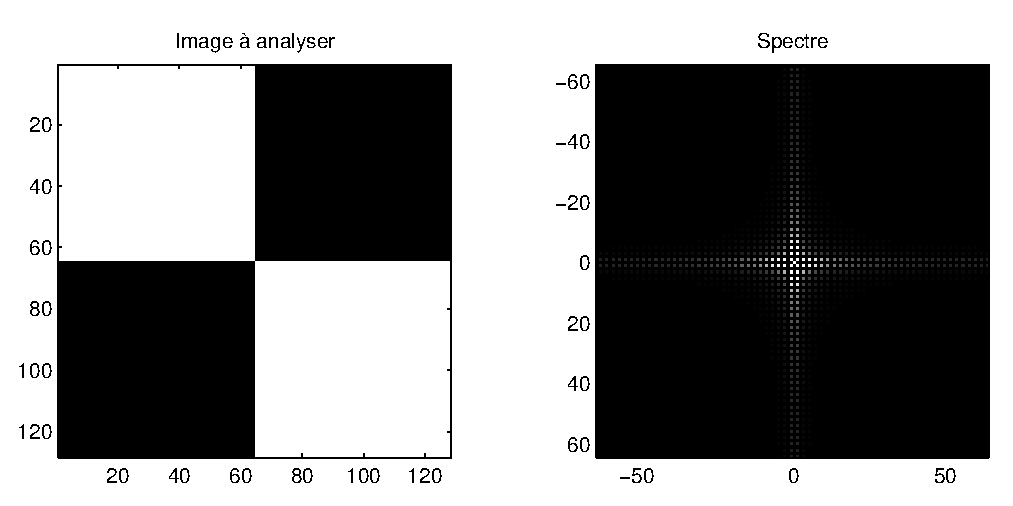
\includegraphics [scale = 0.6]{images/tfd-2d.eps}
    \end{center}
    \caption{2D Fourier transform}
              \label{fig-tfd-2d}
\end{figure}
 
% ------------------------------------------------- -----
% ------------------------------------------------- -----
% sub-section - 2D Convolution                            
% ------------------------------------------------- -----
% ------------------------------------------------- -----
\subsection{2D convolution}
\label{sect2-convolution-2d} 
 
 
\index{Convolution!2D} The convolution between two two-dimensional signals is a direct generalization of the cyclic convolution described in Section~\ref{sect1-convolution-circular}. Once again, we can keep in memory the definition of convolution over a finite group (defined in paragraph \ref{sect2-convolution-transforme-fourier}). This is of course to consider the group $ G \eqdef \ZZ/N \ZZ \times \ZZ/P \ZZ $. We can then interpret the functions of $ \CC [G] $ as images of size $ N \times P $, which we would have extended by periodicity along the two axes. Here is the definition of convolution between two two-dimensional signals. We check that this is an immediate translation of the definition given in the framework of finite abelian groups.
 
\begin{defn}[Two-dimensional convolution]
Let $ f $ and $ g $ be two samples of size $ N \times P $. We define their cyclic convolution product $ f * g $, which is a matrix of size $ N \times P $, as follows:
\begin{equation}
\label{eq-defn-product-convol-2d}
(f * g) [i, \, j] \eqdef \sum_{k = 0}^{N-1}{\sum_{l = 0}^{P-1}{f[k, \, l] g [ik, \, jl]}},
\end{equation}
for $ i \in \{0, \ldots, \, N-1\} $ and $ j \in \{0, \ldots, \, P-1\} $. Of course, all the operations on the indices must be carried out modulo $N$ (resp. $ P $) for the indices on the left (resp. On the right).
\end{defn}
 
 
 
A naive calculation of the convolution product directly by the formula \eqref{eq-defn-product-convol-2d} requires $ (NP)^2 $ operations. In order to quickly calculate such a product, it is necessary to use the algebra morphism property of the Fourier transform on a finite group, which is recalled here in the context of the 2D Fourier transform.
 
\begin{prop}[2D and TFD convolution]
\label{prop-convol-tfd-2d}
Let $ f $ and $ g $ be two samples of size $ N \times P $. We have the convolution formula
\begin{equation}
\label{eq-formula-convolution-tfd-2d}
\forall i \in \{0, \ldots, \, N-1\}, \; \forall j \in \{0, \ldots, \, P-1\}, \quad \wh{f * g}[i, \, j] = \wh{f}[i, \, j] \wh{g}[i, \, j].
\end{equation}
\end{prop}
\begin{proof}
The proof is the exact copy of that of the proposition \ref{prop-convol-tfd}. It is simply necessary to change the cardinal of the group (which is worth $ NP $ and no longer $N$), and to use an indexing adapted for the characters and the indices of the samples, i.e. $ i \in \{0, \ldots, \, N-1\} $ and $ j \in \{0, \ldots, \, P-1\} $.
\end{proof}
This theorem suggests, in order to calculate a convolution, to use the technique to which we are starting to be accustomed. First, you have to calculate the DFTs of the two signals you want to combine. Then, we must multiply them point to point, and finally calculate the inverse transform of the signal obtained. Be careful with the fact that to implement this algorithm, it is necessary to move the entries of negative indices in the two signals, so as to have a signal $N$ periodic on the abscissas, $ P $ periodic on the ordinates, and with indices $ (i, \, j) $ such as $ i \in \{0, \ldots, \, N-1\} $ and $ j \in \{0, \ldots, \, P-1\} $.
 
 
We will see in paragraph \ref{sect2-filtering-2d}, where we will talk about 2D filtering, what are the \guill{intuitive} properties of cyclic convolution, as well as immediate applications to image analysis. We can however give an example of convolution on functions represented by their graph in 3D. Thus the figure \figref{fig-convolution-2d} represents an irregular $ f $ function that we have convolated with a $ g $ function having the shape of a bump (and integral equal to $ 1 $). Convolution has a regularization effect since it realizes a weighted average of the original function in the neighborhood of each point. \begin{figure}[ht]
    \begin{center}
    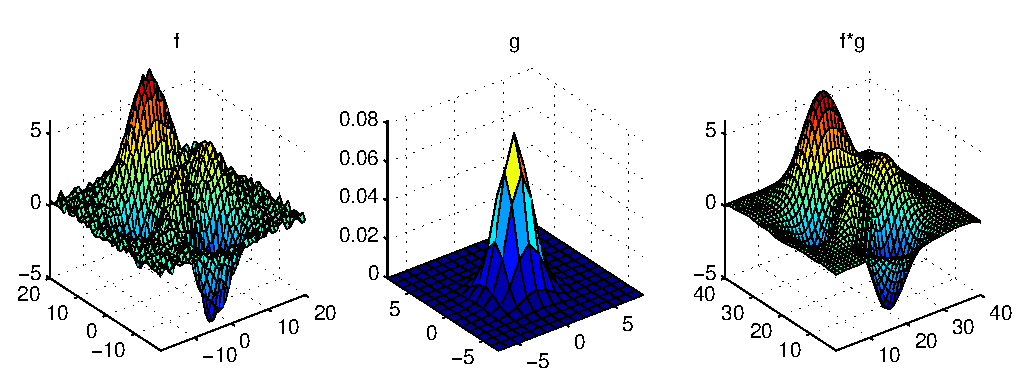
\includegraphics [scale = 0.8]{images/convolution-2d.eps}
    \end{center}
    \caption{2D Convolution}
              \label{fig-convolution-2d}
\end{figure}
 
% ------------------------------------------------- -----
% ------------------------------------------------- -----
% ------------------------------------------------- -----
% section - Symmetry and discrete transform                            
% ------------------------------------------------- -----
% ------------------------------------------------- -----
% ------------------------------------------------- -----
\section{Symmetry and discrete transform}
% \addcontentsline{toc}{section}{Symmetry and discrete transform}
\label{sect1-symetrie-tfd} 
 
\index{Symmetry} In this paragraph, we will give some additional properties of the discrete Fourier transform, and thus create its eigenvectors from given vectors.
% ------------------------------------------------- -----
% ------------------------------------------------- -----
% sub-section - Symmetry properties                            
% ------------------------------------------------- -----
% ------------------------------------------------- -----
\subsection{Symmetry properties}
\label{sect2-prop-symmetry} 
 
Let's start by defining different operations on the functions of $ \ZZ/N \ZZ $ in $ \CC $.
 
\begin{defn}[Symmetry operator]
\label{defn-symmetry-operator}
\index{Operator!of symmetry} \label{notation-48} Let $ f = \{f[0], \ldots, \, f[N-1]\} $ be a vector of size $N$ which we associates a periodic function $ f_1 $, which can be seen as a function $ f_1: \ZZ/N \ZZ \rightarrow \CC $. We define \textit{the symmetrized function} $ f^\sharp $ by:
\begin{equation}
\label{eq-defn-symmetrical-sample}
\forall n \in \{0, \ldots, \, N-1\}, \quad f^\sharp [n] \eqdef f_1 (-n).
\end{equation}
Thus, we have $ f^\sharp = \{f[0], \, f[N-1], \, f[N-2], \ldots, \, f[1]\} $. \\A vector $ f $ is said to be \textit{symmetric} if it satisfies $ f^\sharp = f $. It says \textit{anti-symmetric} if $ f^\sharp = -f $.
\end{defn}
 
 
\begin{defn}[Decomposition]
\label{defn-parts-sym-anti-sym}
\index{Symmetric part} \label{notation-49} For $ f \in \CC^N $, we denote by $ \psym{f} $ and $ \pasym{f} $ the parts \textit{symmetric} and \textit{anti-symmetric} of $ f $, defined by the equations
\begin{align*}
\psym{f} & \eqdef \frac{1}{2} \left(f + f^\sharp \right), \\
\pasym{f} & \eqdef \frac{1}{2} \left(f - f^\sharp \right).
\end{align*}
We have of course the decomposition $ f = \psym{f} + \pasym{f} $.
\end{defn}
 
 
\begin{prop}[Symmetry properties]
Let $ f \in \CC^N $ be a sample. We have the following properties. \begin{itemize}
\item [{\upshape (i)}] $ \Ff(f^\sharp) = N \Ff^{-1} (f) $ as well as $ \Ff^2 (f^\sharp) = N f $ .
\item [{\upshape (ii)}] If $ f $ is symmetric, then $ \Ff^2 (f) = N f $ and $ \Ff(f) $ is symmetric.
\item [{\upshape (iii)}] If $ f $ is anti-symmetric, then $ \Ff^2 (f) = -N f $ and $ \Ff(f) $ is anti-symmetric.
\item [{\upshape (iv)}] If $ f \in \RR^N $ is symmetric, then $ \Ff(f) \in \RR^N $.
\item [{\upshape (v)}] If $ f \in \RR^N $ is anti-symmetric, then $ \Ff(f) \in (\imath \RR)^N $.
\end{itemize}
\end{prop}
\begin{proofnoqed}
We prove (i) and (iv): \\For (i), we have
\begin{equation*}
\Ff(f^\sharp) = \sum_{k \neq 0}{f[-k] \omega_N^{- kn}} + f[0] = \sum_{k = 0}^{N-1}{f[k] \omega_N^{kn}} = \Ff(f) [n].
\end{equation*}
For (iv), if we denote by $ \ol{z} $ the conjugate of $ z \in \CC $, we have
\begin{equation*}
\ol{\Ff(f) [n]} = \sum_{k}{\ol{f[k]} e^{+ \frac{2 \imath \pi}{N} kn}} = \sum_{k}{f^\sharp [k] e^{\frac{2 \imath \pi}{N} kn}} = \Ff(f^\sharp) [n] = \Ff(f) [n]. \tag *{\qed}
\end{equation*}
\end{proofnoqed}
 
% ------------------------------------------------- -----
% ------------------------------------------------- -----
% sub-section - Eigenvalues of the TFD                            
% ------------------------------------------------- -----
% ------------------------------------------------- -----
\subsection{Eigenvalues of the TFD}
\label{sect2-eigenvalues-tfd} 
 
\index{Unit!Matrix} The study of a linear operator is greatly facilitated by the knowledge of its eigenvalues and the associated eigenvectors. Although the $ \frac{1}{\sqrt{N}} \Omega_N $ matrix is arguably the most important unit matrix, finding its eigenvectors is a difficult subject. We will now give a simple way to construct eigenvectors of the DFT.
 
\begin{thmdefn}
\index{Eigenvector} \index{Eigenvalue} Let $ f \in \CC^N $ be a sample. We define
\begin{align*}
& \Uu_+ (f) \eqdef \sqrt{N} \psym{f} + \Ff(\psym{f}) \quad \quad \text{and} & \Uu_- (f) \eqdef \sqrt{N} \psym{f} - \Ff(\psym{f}) \\
& \Vv_+ (f) \eqdef \sqrt{N} \pasym{f} + \imath \Ff(\pasym{f}) \quad \quad \text{and} & \Vv_- (f) \eqdef \sqrt{N} \pasym{f} - \imath \Ff(\pasym{f}).
\end{align*}
We then have
\begin{align*}
& \Ff(\Uu_+ (f)) = \sqrt{N} \Uu_+ (f) \quad \text{et} \quad \Ff(\Uu_- (f)) = - \sqrt{N} \Uu_- (f) \\
& \Ff(\Vv_+ (f)) = - \imath \sqrt{N} \Vv_+ (f) \quad \text{et} \quad \Ff(\Vv_- (f)) = \imath \sqrt{N} \Vv_- (f).
\end{align*}
This means that the vectors $ \Uu_+ (f) $, $ \Uu_- (f) $, $ \Vv_+ (f) $ and $ \Vv_- (f) $ are \textit{eigenvectors} of the discrete Fourier transform.
\end{thmdefn}
\begin{proof}
Let's prove the first equality: $ \Ff(\Uu_+ (f)) = \sqrt{N} \Ff(\psym{f}) + \Ff^2 (\psym{f}) $. And since $ \psym{f} $ is symmetric, we have $ \Ff^2 (\psym{f}) = N \psym{f} $, hence the result.
\end{proof}
 
 
\begin{rem}
We can add that the \textit{eigenvalues} that we have just found are the only ones, since the Fourier transform satisfies $ \Ff^4 (f) = N f $. So its eigenvalues are necessarily \ordin{4}{th} roots of $ N^2 $.
\end{rem}
\index{Eigenvector} \index{Eigenvalue} \index{Fourier transform!partial} \index{Operator square root} Figure \figref{fig-square-root-tfd} shows the different constructed eigenvectors from the function that can be seen on the left of the figure \figref{fig-root-interm-tfd} (that is to say for $ \lambda = 0 $). \begin{figure}[ ht] 
    \begin{center}
    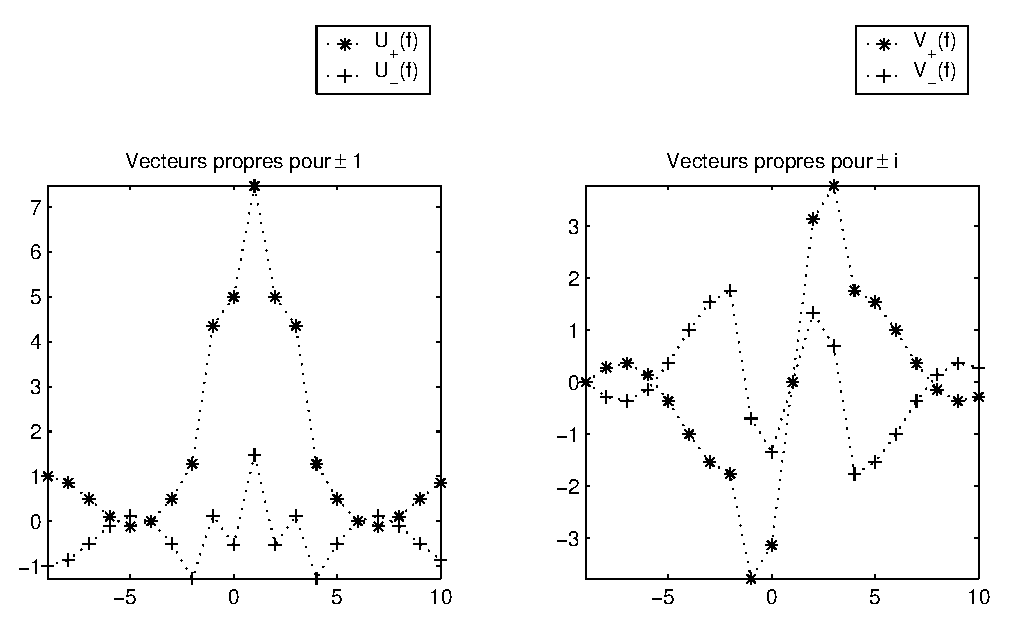
\includegraphics [scale = 0.6]{images/racine-carree-tfd.eps}
    \end{center}
    \caption{Eigenvectors $ \Uu_+ (f), \, \Uu_- (f), \, \Vv_+ (f) $ and $ \Vv_- (f) $}
              \label{fig-square-root-tfd}
\end{figure}
This proposition allows an interesting construction, simply by writing the decomposition of a vector $ f \in \CC^N $ as a function of the eigenvectors of the Fourier transform:
\begin{equation*}
f = \Uu_+ (f) + \Uu_- (f) + \Vv_+ (f) + \Vv_- (f).
\end{equation*}
This allows to consider the operator $ \sqrt{\Ff} $ defined as follows:
\begin{equation*}
\sqrt{\Ff} (f) \eqdef N^{1/4} \Uu_+ (f) + \imath N^{1/4} \Uu_- (f) + (- \imath)^{1 / 2} N^{1/4} \Vv_+ (f) + \imath^{1/2} N^{1/4} \Vv_- (f),
\end{equation*}
where we have chosen for $ \imath^{1/2} $ a \textit{square root} of $ \imath $ (arbitrary choice).
 
We then have $ \sqrt{\Ff} \circ \sqrt{\Ff} = \Ff $: the operator $ \sqrt{\Ff} $ is a square root of the discrete Fourier transform. Likewise, for $ \lambda \in \RR $, we can thus construct $ \Ff^\lambda $, a \ordin{\lambda}{ième} transform of $ \Ff $ (again, the construction n' is absolutely nothing canonical). Figure \figref{fig-root-interm-tfd} shows different intermediate transforms. For $ \lambda = 0.5 $ we get $ \sqrt{\Ff} $. \begin{figure}[ht]
    \begin{center}
    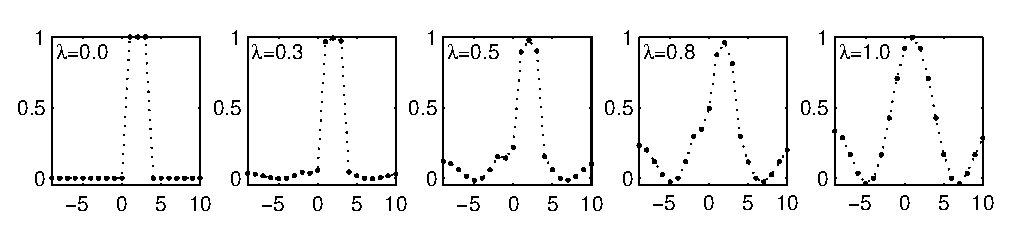
\includegraphics [scale = 0.7]{images/racine-interm-tfd.eps}
    \end{center}
    \caption{Intermediate transformed vectors $ \Ff^\lambda (f) $ for $ \lambda \in [0,1] $}
              \label{fig-root-interm-tfd}
\end{figure}
The exercise \oldref{exo-transforme-partial-fourier} allows to handle a \textit{partial Fourier transform}, which generalizes the construction that we have just performed. We can see, thanks to the example of a Gaussian, that these manipulations correspond to very intuitive notions. For more information on the partial Fourier transform (continuous as well as discrete), one can consult the article of \nompropre{Cariolaro} \cite{cariolaro-partial-fourier}. Finally, the exercise \oldref{exo-diagonalization-tfd} proposes a method to canonically diagonalize the matrix of the TFD.

% ------------------------------------------------- -----
% ------------------------------------------------- -----
% ------------------------------------------------- -----
% section - Exercises                            
% ------------------------------------------------- -----
% ------------------------------------------------- -----
% ------------------------------------------------- -----
\section{Exercises}
% \addcontentsline{toc}{section}{Exercises}
\label{sect1-chap2-exercises} 
 
 
 
\begin{exo}[Bit inversion]
\label{exo-bit-reversal}
 
\index{Bit inversion} We define, for $ n \geq 0 $, vectors $ u^{(n)} $ of size $ 2^n $, by $ u^{(0)} = \{0\} $ and
\begin{equation*}
\forall n> 0, \; \forall k \in \{0, \ldots, \, 2^n-1\}, \quad u^{(n)}[k] \eqdef \left\{\begin{array}{ll} 2 u^{(n-1)}[k] & \text{si} k <2^{n-1} \\2 u^{(n-1)}[k-2^{n-1}] + 1 & \text{si} k \geq 2^{n-1} \end{array} \right. .
\end{equation*}
\begin{enumerate}
\item Calculate the value of $ u^{(n)} $ for $ n = 1, \, 2, \, 3 $.
\item Show that $ u^{(n)} $ is in fact the sequence $ 0, \ldots, \, 2^n-1 $, classified by considering the reverse binary writes of the inputs.
\item Let $ f $ be a vector of size $ 2^n $. We denote by $ \wt{f} $ the sequence determined by
\begin{equation*}
\forall k \in \{0, \ldots, \, 2^n-1\}, \quad \wt{f}[k] \eqdef f[u^{(n)}[k]].
\end{equation*}
What is the use of $ \wt{f} $ when computing the discrete Fourier transform of $ f $?
\item We denote by $ f^0 $ and $ f^1 $ the even and odd parts of $ f $. We denote by $ \wt{f}_d $ and $ \wt{f}_g $ the left and right parts of $ \wt{f} $. What relation binds all these vectors?
\item \index{Matlab@\Matlab{}} \index{Complexity} Implement in \Matlab{} a recursive algorithm to calculate $ \wt{f} $. Compare its complexity to that of the \texttt{\upshape rev \_bits} procedure.
\end{enumerate}
\end{exo}
 
 
\begin{exo}[Good-Thomas algorithm]
\label{exo-algo-good-thomas}
 
\index{Good-Thomas@\nompropreindex{Good-Thomas}} \index{Cooley-Tukey@\nompropreindex{Cooley-Tukey}} \index{Algorithm!of Good-Thomas} We saw in paragraph \ref{sect2-transfo-cooley-tukey} that the FFT algorithm of \textit{Cooley-Tukey} generalized without problem if we had an adequate factorization of $N$, the size of the transformed vector. In this exercise, we will see that if some integers of this factorization are coprime, we can design an even faster algorithm. \begin{enumerate}
\item \index{Ring} \index{Ring!morphism} \index{Chinese!lemma} We assume that $ N = p \, q $ where $ p $ and $ q $ are two prime numbers to each other. We recall the \textit{Chinese lemma}, which says that the application
\begin{equation*}
\varphi \func{\ZZ/N \ZZ}{\ZZ/p \ZZ \times \ZZ/q \ZZ}{n}{(n \mod p, \, n \mod q)}
\end{equation*}
is an isomorphism of rings. Explain the inverse morphism $ \psi $.
\item Let $ f \in \CC^N $. We then define a 2D signal:
\begin{equation*}
\forall k_1 \in \{0, \ldots, \, p-1\}, \; \forall k_2 \in \{0, \ldots, \, q-1\}, \quad F [k_1, \, k_2] \eqdef f[\psi (k_1, \, k_2)].
\end{equation*}
Show that we have
\begin{equation*}
\wh{f}[(s_1 q + s_2 p) \mod N] = \wh{F}[s_1, \, s_2].
\end{equation*}
 
\item Show that when $ s_1 $ traverses $ \{0, \ldots, \, p-1\} $ and $ s_2 $ traverses $ \{0, \ldots, \, q-1\} $, then $ ( s_1 q + s_2 p) \mod N $ iterates $ \{0, \ldots, \, N-1\} $. Deduce how we can calculate the Fourier transform of $ f $ from that of $ F $, by explaining the change of indices.
\item What is the gain compared to a step of the classic FFT algorithm? In particular, what becomes of the operator $ \Ss_N^x $ introduced to the equation \eqref{eq-operator-S}? Propose a recursive procedure which, following the factorization of $N$ obtained at each step, calls the optimal DFT calculation procedure. In addition to the FFT procedures of Cooley-Tukey and Good-Thomas, we can include the Chirp procedure described in the exercise \oldref{exo-chirp-transform-finis-corps}, which is interesting when $ N-1 $ is a Prime number.
\end{enumerate}
\end{exo}
 
 
\begin{exo}[Split-Radix algorithm]
\label{exo-algo-split-radix}
 
\index{Algorithm!split-radix} \index{Split-radix} \index{Twiddle factor} \index{Decimation!frequency} We saw in paragraph \ref{sect2-variations-fft} that it was possible to extend the Cooley-Tukey dichotomy method to compute DFTs of length $ p^r $, by grouping inputs by packets of size $ p $. In this exercise, we will show how, by cleverly choosing packets of varying sizes, we can reduce the number of operations. This choice starts from the observation that the Cooley-Tukey algorithm spends a lot of time calculating the operator $ \Ss_N^x $, whereas for some values of $N$ (for example $ 2 $ or $ 4 $), this last is trivial. In Anglo-Saxon literature, the roots of the unit added by this operator are called \guill{twiddle factors} (literally, \guill{twiddling their thumbs}). We can compare this approach with that of the Good-Thomas algorithm, exercise \oldref{exo-algo-good-thomas}, which in the context of a certain factorization of $N$, eliminates the operator $ \Ss_N^x $. \begin{enumerate}
\item We consider a frequency decimation scheme. Assume that $N$ is a power of $ 2 $. It is recalled that the classical DIF algorithm organizes the following grouping:
\begin{align*}
\enscond{\wh{f}[k]}{k = 0, \ldots, \, N-1} = & \enscond{\wh{f}[2 k]}{k = 0, \ldots, \, \ofrac{N}{2}-1} \bigcup \\
& \enscond{\wh{f}[2 k + 1]}{k = 0, \ldots, \, \ofrac{N}{2}-1}.
\end{align*}
Explain why there is no interest in touching the first part of this grouping. Regarding the second part, we propose the grouping corresponding to base 4 transforms, that is to say:
\begin{align*}
\enscond{\wh{f}[2 k + 1]}{k = 0, \ldots, \, \ofrac{N}{2}-1} = & \enscond{\wh{f}[4 k + 1]}{k = 0, \ldots, \, \ofrac{N}{4}-1} \bigcup \\
& \enscond{\wh{f}[4 k + 3]}{k = 0, \ldots, \, \ofrac{N}{4} -1}
\end{align*}
Show that this leads to the following transformation formulas:
\begin{equation*}
\wh{f}[4k + 2j + 1] = \sum_{n_1 = 0}^{\frac{N}{4} -1}{\omega_{N / 4}^{- k n_1} \omega_N^{-n_1 (2j + 1)} \sum_{n_2 = 0}^{3}{f \left[n_1 + n_2 \ofrac{N}{4} \right] \omega_4^{- n_2 (2j + 1) }}},
\end{equation*}
for $ j = 0, \, 1 $ and $ k = 0, \ldots, \, \frac{N}{4} -1 $. Are domestic sums complicated to calculate? Identify the \guill{twiddle factors}.
\item Find other grouping schemes. Why is grouping by 4 advantageous? Calculate the number of operations required each time, and compare with that of the classic DIF diagram, in base 2.
\item Transform the algorithms described above to obtain a temporal decimation scheme (grouping of inputs). Describe an iterative implementation of the algorithms, not forgetting the bit reversal procedures allowing to save temporary memories.
\end{enumerate} For more information, and a generalization to DFTs of length $ p^r $, we can consult{\upshape \cite{vetterli-split-radix}}.
\end{exo}
 
 
\begin{exo}[Optimized convolution]
\label{exo-calcul-convolution-fft}
 
\index{Convolution!acyclic} We want to compute the acyclic convolution of two finite sequences $ f $ and $ g $ of respective sizes $N$ and $ M $. Assume that $ M $ is much smaller than $N$. For simplicity, suppose that the indices of the two sequences start at $ 0 $. \begin{enumerate}
\item We take $ N = p M $. We denote by $ f_j \eqdef \{f[k + j M]\}_{k = 0}^{M-1} $, for $ j = 0, \, \ldots, \, p -1 $. Show that we have
\begin{equation*}
f \star g [k] = \sum_{j = 0}^{p-1}{f_j \star g [k - j M]}.
\end{equation*}
 
\item \index{Complexity} Deduce a quick way to calculate $ f \star g $ without having to add $ NM-1 $ zeros at the end of $ g $. What is the complexity of the algorithm obtained?
\item If $N$ is not a multiple of $ M $, what can be done?
\end{enumerate}
\end{exo}
 
 
\begin{exo}[Circulating matrix]
\label{exo-circulating-matrix}
 
\index{Matrix!circulating} \index{Determinant!circulating} This exercise has strong similarities with the exercise \oldref{exo-determinant-circulating} on circulating determinants, with a presentation this time using the convolution product. Let $ c \eqdef \transp{(c_0, \ldots, \, c_{N-1})} \in \CC^N $ be a vector of size $N$. We define the circulating matrix $ C $ which is associated with this vector by
\begin{equation*}
C \eqdef \begin{pmatrix} c_0 & c_{N-1} & c_{N-2} & \ldots & c_{1} \\c_1 & c_0 & c_1 & \ldots & c_{2} \\\vdots & \vdots & \vdots & & \vdots \\c_{N-1} & c_{N-2} & c_{N-3} & \ldots & c_{0} \end{pmatrix}.
\end{equation*}
\begin{enumerate}
\item Let $ \{e_1, \ldots, \, e_N\} $ be the canonical basis of $ \CC^N $. We consider the matrix $ R $ whose columns are $ \{e_2, \, e_3, \ldots, \, e_N, \, e_1\} $. We recall that $ \Omega_N $ designates the Fourier matrix, which is defined by the equation \eqref{eq-defn-matrix-fourier}. Show that we have
\begin{equation*}
\Omega_N R \Omega_N^{-1} = D \quad \quad \text{with} \quad D = \diag (1, \, \omega_N^{-1}, \ldots, \, \omega_N^{- (N-1)}).
\end{equation*}
 
\item Show while we have
\begin{equation*}
\Omega_N C \Omega_N^{-1} = \Delta \quad \quad \text{with} \quad \Delta = \diag (\wh{c}[0], \, \wh{c}[1], \ldots, \, \wh{c}[N-1]).
\end{equation*}
Deduce that for $ x \in \CC^N $, we can calculate the product $ C x $ as follows:
\begin{equation*}
C x = \Omega_N^{-1} \left((\Omega_N c) \cdot (\Omega_N x) \right),
\end{equation*}
where we denote by $ \cdot $ the product component by component of the matrices.
\item Show that for $ x \in \CC $, we have $ C x = c * x $. Using the convolution theorem \ref{prop-convol-tfd}, deduce an immediate proof of the previous question.
\end{enumerate}
\end{exo}
 
 
\begin{exo}[Trigonometric interpolation]
\label{exo-interpolation-trigonometric}
\index{Interpolation!trigonometric} \index{Zero padding} Let $ f \in \CC^N $ be a sample of size $ N = 2N_0 + 1 $. We define a vector $ f_0 $ of size $ P = \eta N $ (with $ \eta \in \NN $ sufficiently large) as follows:
\begin{equation*}
\wh{f_0} \eqdef \eta \left\{\wh{f}[0], \, \wh{f}[1], \ldots, \, \wh{f}[N_0], \, 0 , \ldots, \, 0, \, \wh{f}[N_0 + 1], \ldots, \, \wh{f}[N-1] \right\}.
\end{equation*}
Show that we have
\begin{equation*}
\forall k \in \{0, \ldots, \, N-1\}, \quad f[k] = f_0 [\eta k].
\end{equation*}
Deduce a fast algorithm to interpolate a function by trigonometric polynomials. We can see this algorithm in action in figure \figref{fig-fft-interpolation}. \begin{figure}[ht]
    \begin{center}
    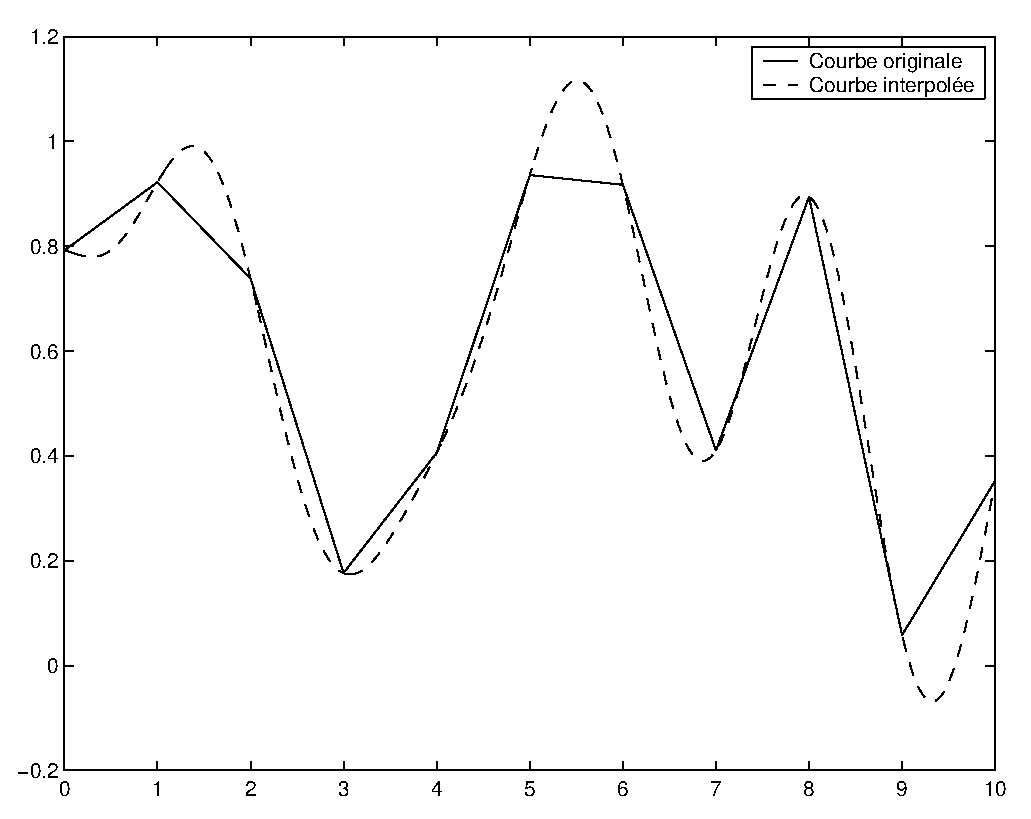
\includegraphics [scale = 0.4]{images/fft-interpolation.eps}
    \end{center}
    \caption{Trigonometric interpolation}
              \label{fig-fft-interpolation}
\end{figure}f
\end{exo}
 
 
\begin{exo}[Chebyshev interpolation]
\label{exo-interpolation-chebyshev}
\index{Chebyshev@\nompropreindex{Chebyshev}} \index{Polynomial!of Chebyshev} \index{Transform!into cosine} \index{Runge phenomenon} \index{Interpolation!of Chebyshev} \index{Interpolation!of Lagrange} \index{Lissajou curve} We define the polynomials of \textit{Chebyshev} by
\begin{equation*}
T_k (X) \eqdef \cos (k \arccos (X)).
\end{equation*}
The figure \figref{fig-polynomes-chebyshev} shows the graphical representations of the polynomials $ T_k $ for small values of $ k $. These are special cases of Lissajou figures (which are used to study wave phenomena), i.e. parameterized curves of the type $ (x = a \cos (kt + c), \, y = b \cos (t)) $. \begin{figure}[ht]
    \begin{center}
    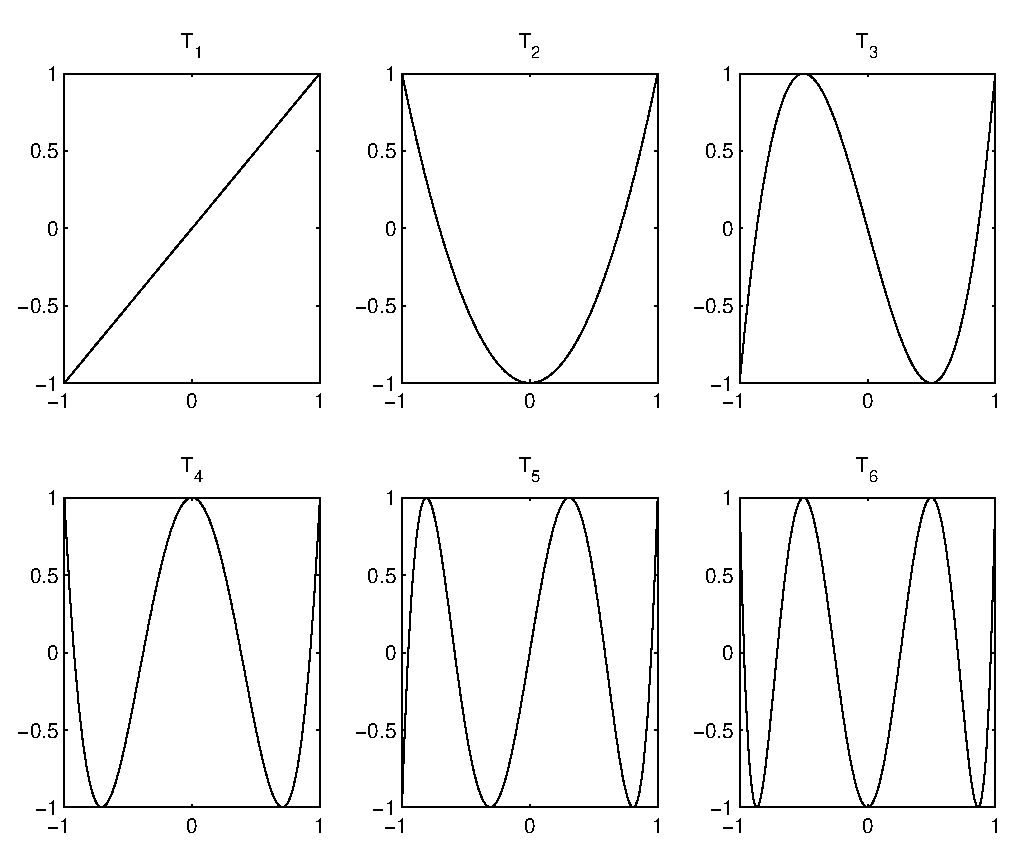
\includegraphics [scale = 0.6]{images/polynomes-chebyshev.eps}
    \end{center}
    \caption{Polynomials $ T_k $ for $ k = 1, \ldots, \, 6 $}
              \label{fig-polynomes-chebyshev}
\end{figure}
We consider a continuous function $ f: [-1,1] \rightarrow \RR $. We want to interpolate it in $N$ points $ \{x_k\}_{k = 0}^{N-1} $ by a polynomial $ P_{N-1} $ of degree $ N-1 $, where the $ x_k $ are defined by
\begin{equation*}
\forall k \in \{0, \ldots, \, N-1\}, \quad x_k \eqdef \cos \left((k + 1/2) \frac{\pi}{N} \right).
\end{equation*}
\begin{enumerate}
\item Show that $ T_N $ is indeed a polynomial, by determining a recurrence relation between $ T_k $ and $ T_{k-1} $. Show that the roots of $ T_N $ are $ x_k $, for $ k \in \{0, \ldots, \, N-1\} $.
\item Show that $ P_{N-1} $ can be put in the form
\begin{equation*}
P_{N-1} = \sum_{k = 0}^{N-1}{\alpha_k T_k}.
\end{equation*}
 
\item \index{Compression!JPEG} \index{JPEG} \index{Inversion formula} We consider two types of discrete cosine transforms (often denoted DCT-2 and DCT-3 in English, because there are d'others) of a sample $ \{f[k]\}_{k = 0}^{N-1} \in \RR^N $:
\begin{align*}
\Cc_2 (f) [j] & \eqdef \sum_{k = 0}^{N-1}{f[k] \cos \left((k + 1/2) \frac{j \pi}{N } \right)} \\
\Cc_3 (f) [j] & \eqdef \frac{1}{2} f[0] + \sum_{k = 1}^{N-1}{f[k] \cos \left((j + 1/2) \frac{k \pi}{N} \right)}.
\end{align*}
\index{Matlab@\Matlab{}} Show that the inverse of $ \Cc_2 $ is $ \frac{2}{N} \Cc_3 $. Implement in \Matlab{} these transforms using a DFT of size $ 4N $ (we can think of making the signal even, then inserting 0 at odd indices). For more information on the cosine transform, we can consult the article of \nompropre{Strang}{\upshape \cite{strang-dct}}. Note that it is the transform $ \Cc_2 $ which is used for the compression of JPEG images.
\item How to calculate the $ \{\alpha_k\}_{k = 0}^{N-1} $ from $ \{f[k] = f(x_k)\}_{k = 0}^{N-1} $? Conclude a fast polynomial interpolation algorithm at the points $ x_k $.
\end{enumerate} The figure \figref{fig-interpolation-chebyshev} shows a comparison between the Lagrange interpolation (equidistant points) and the Chebyshev interpolation on a seemingly innocuous function:
\begin{equation*}
f(x) \eqdef \frac{1}{\alpha^2 + x^2} \quad \text{for} \quad \alpha \in \RR^*_+.
\end{equation*}
For the figure, we have taken $ N = 11 $, and $ \alpha = 0.3 $. Try, experimentally, to determine the value $ \alpha_0 $ from which the Lagrange polynomial uniformly converges to $ f $ when $ n \rightarrow + \infty $. \begin{figure}[ht]
    \begin{center}
    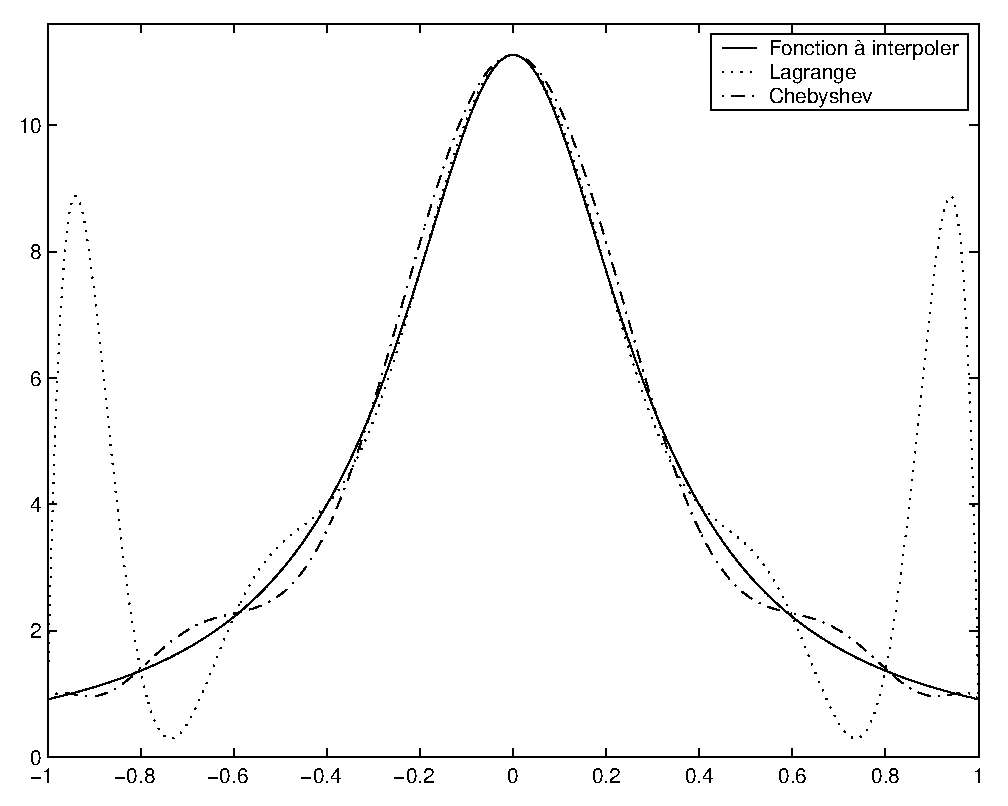
\includegraphics [scale = 0.4]{images/interpolation-chebyshev.eps}
    \end{center}
    \caption{Lagrange and Chebyshev interpolation}
              \label{fig-interpolation-chebyshev}
\end{figure}
\index{Method!spectral} Chebyshev interpolation is a simple case of spectral method. These methods use decompositions according to orthogonal polynomials to approximate the solutions of partial differential equations. This is an extension of Fourier series decompositions adapted to non-periodic functions. This is all very well described in \nompropre{Boyd}{\upshape \cite{boyd-spectral}}.
\end{exo}
 
 
\begin{exo}[Fractional derivation]
\label{exo-derivation-fractionionnaire}
 
\index{Fractional derivation} Let $ f: \RR \rightarrow \RR $ be a function of class $ \CC^\infty $ rapidly decreasing to infinity. Show that the Fourier transform (defined by the equation \eqref{eq-transforme-fourier-R}) of $ f^{(n)} $ is
\begin{equation*}
\Ff(f^{(n)}) (\xi) = (- \imath \xi)^{- n} \Ff(f) (\xi).
\end{equation*}
Explain how this property allows us to define a \textit{fractional derivation}, ie we can define a derivation for real values of $ n $. Implement a \Matlab{} routine which performs an approximate fractional derivative calculation using the FFT algorithm. The figure \figref{fig-derivation-fractionionnaire} shows the fractional derivative of a Gaussian obtained by this method, and this for different values of $ n $ between 0 and 2. \begin{figure}[ht]
    \begin{center}
    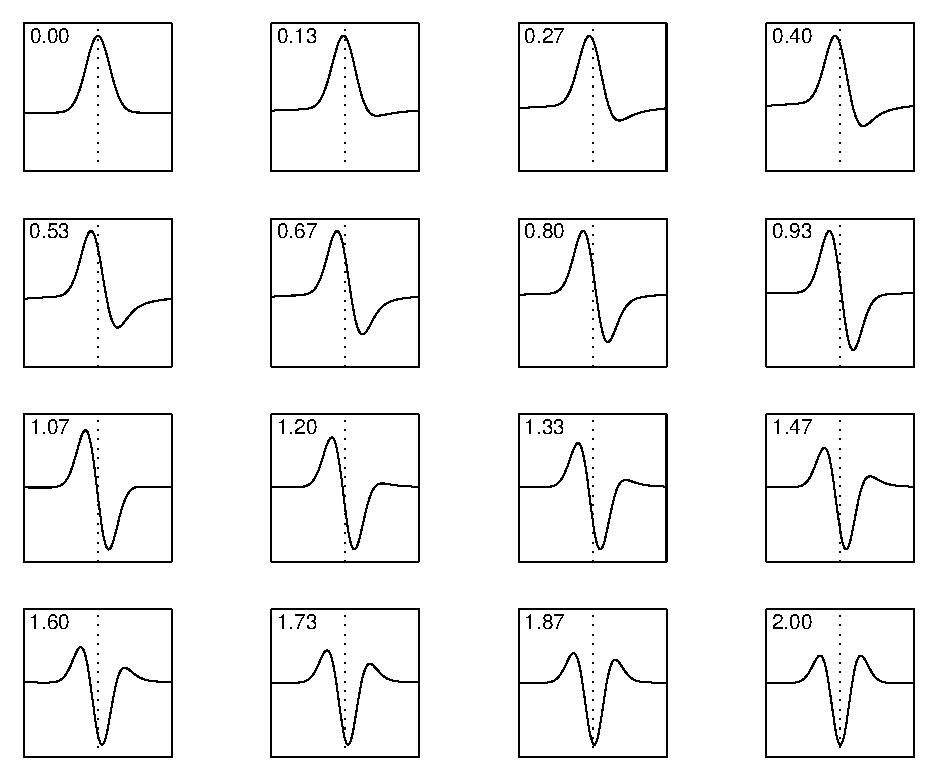
\includegraphics [scale = 0.5]{images/derivation-fractionnaire.eps}
    \end{center}
    \caption{Successive fractional derivatives of a Gaussian}
              \label{fig-derivation-fractionionnaire}
\end{figure}
\end{exo}
 
 
\begin{exo}[Intermediate Fourier transform]
\label{exo-transforme-partial-fourier}
 
\index{Fourier!intermediate!transform} \index{Normal!Endomorphism} \index{Unit!Endomorphism} \index{Unit!matrix} \index{Diagonalization} \index{Fourier!intermediate!Transform} We recall that we Note $ \Omega_N $ the Fourier matrix, which is defined by the equation \eqref{eq-defn-matrix-fourier}. It is a self-joined matrix, so like any normal endomorphism (i.e. which commutes with its adjunct), it diagonalizes to the orthonormal basis of $ \CC^N $ (which is false in $ \RR^N $). This means that there exists a unitary $ P $ matrix and a diagonal $ D $ matrix such that
\begin{equation*}
\Omega_N = PDP^{*}.
\end{equation*}
\begin{enumerate}
\item What are the entries of $ D $? Check this with \Matlab{}, by using the command \texttt{eig} which provides the eigenvalues as well as a decomposition according to the eigenvectors. It will be noticed that as the number of distinct eigenvalues is lower than $N$, the choice of the orthonormal basis of eigenvectors is totally arbitrary.
\item We define the matrix $ \Omega_N^{\alpha} $, for $ \alpha \in \RR $, by
\begin{equation*}
\Omega_N^{\alpha} \eqdef PD^{\alpha} P^{*},
\end{equation*}
where $ D^{\alpha} $ is \textit{one} power \ordin{\alpha}{th} of $ D $. We then define intermediate Fourier transforms:
\begin{equation*}
\forall f \in \CC^N, \quad \Ff^{\alpha} (f) \eqdef \Omega_N^{\alpha} f.
\end{equation*}
Show that we have
\begin{equation*}
\forall (\alpha, \beta) \in \RR^2, \quad \Ff^{\alpha} \circ \Ff^{\beta} = \Ff^{\alpha + \beta} \quad \text{and} \quad \Ff^1 = \Ff.
\end{equation*}
 
\item The figure \figref{fig-matrix-partial-tfd} shows the modulus of the matrix $ \Ff^{\alpha} $ for a parameter $ \alpha $ varying between $ 0.3 $ and $ 1 $. What do the two white diagonals that we can distinguish represent (we can use the calculation of the matrix $ \Omega_N^2 $)? 

\begin{figure}[ht]
    \begin{center}
    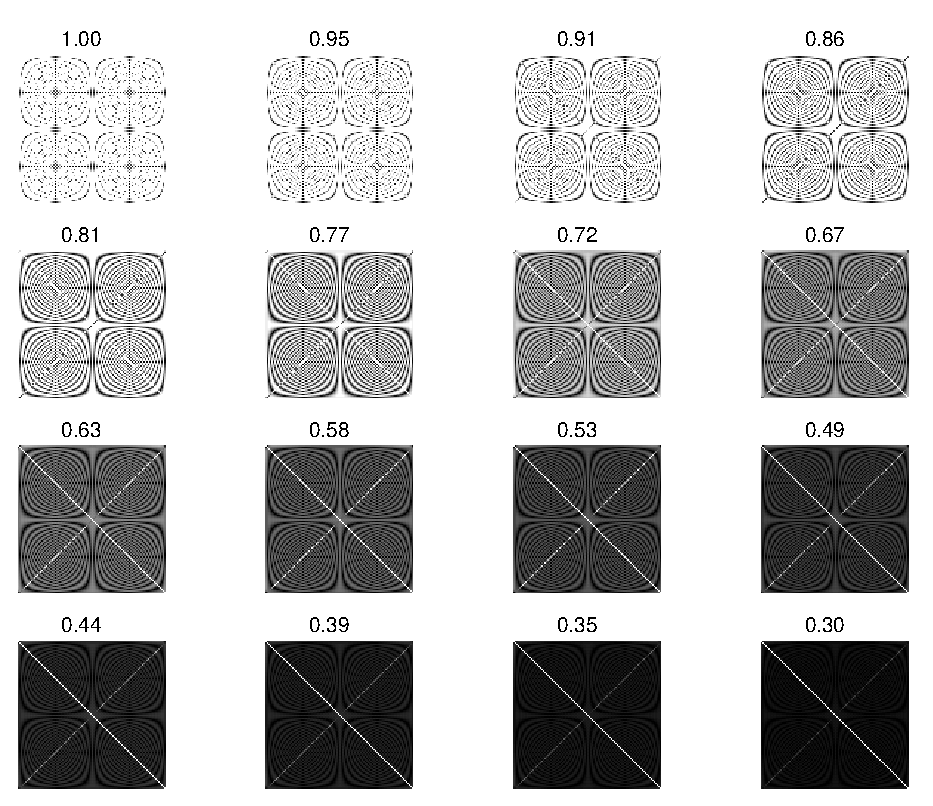
\includegraphics [scale = 0.5]{images/matrice-tfd-partielle.eps}
    \end{center}
    \caption{Modulus of different partial Fourier transform matrices}
              \label{fig-matrix-partial-tfd}
\end{figure}
 
\item Explain why we can construct an infinite number of intermediate transforms. By letting \Matlab{} decide on a factorization of $ \Omega_N $, implement the obtained transform, then test it with different values of $ \alpha $ and different signals.
\end{enumerate} Figure \figref{fig-transforme-partial-fourier} shows a panel of intermediate transforms for a Gaussian. The $ \alpha $ transformation parameter varies between $ 0 $ and $ 2 $. Of course, for $ \alpha = 2 $, we find the original signal (because the Gaussian is symmetrical). 

\begin{figure}[ht]
    \begin{center}
    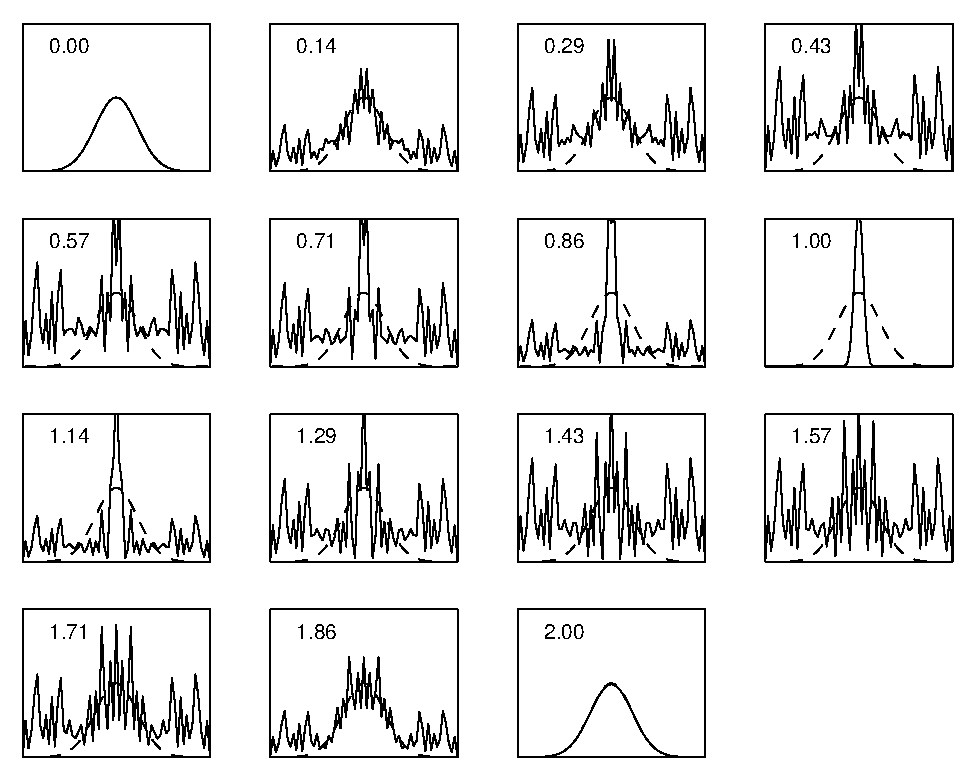
\includegraphics [scale = 0.5]{images/transformee-fourier-partielle.eps}
    \end{center}
    \caption{Successive partial Fourier transforms of a Gaussian}
              \label{fig-transforme-partial-fourier}
\end{figure}
\end{exo}
 
 
\begin{exo}[Diagonalization of the TFD]
\label{exo-diagonalization-tfd}
 
\index{Diagonalization} \index{Orthonormal basis} \index{Eigenvector} In the previous exercise, we used \Matlab{} to diagonalize the matrix of the TFD into orthonormal basis. The theoretical construction of an orthonormal basis is not simple, mainly because the eigenvalues have a multiplicity greater than 1, which leaves a potentially infinite choice of decompositions. The goal is therefore to build a canonical process to determine a basis for diagonalization. This exercise is inspired by the article by \nompropre{Dickinson}{\upshape \cite{dickinson-eigenvectors}}. We can also read the article of \nompropre{Candan}{\upshape \cite{candan-fractional}} which makes the relation between the matrix $ S $ and the discretization of a differential equation. \begin{enumerate}
\item \label{notation-50} \label{notation-51} We define a matrix $ S \in M_N (\RR) $ as follows:
\begin{equation*}
S \eqdef \begin{pmatrix} C_0 & 1 & 0 & \ldots & 1 \\1 & C_1 & 1 & \ldots & 0 \\0 & 1 & C_2 & \ldots & 0 \\\vdots & \vdots & \vdots & \ddots & \vdots \\1 & 0 & 0 & \ldots & C_{N-1} \end{pmatrix} \quad \text{where} \quad C_k \eqdef 2 \left(\cos \left(\frac{2k \pi}{N} \right) - 2 \right).
\end{equation*}
Explain why $ S $ diagonalizes in orthonormal basis.
\item \index{Circulating!Matrix} Show that $ S $ and $ \Omega_N $, the Fourier matrix, commute, that is, $ S \Omega_N = \Omega_N S $. We can decompose $ S $ into $ S = \Gamma + \Delta $, where $ \Gamma $ is a circulating matrix cleverly chosen so that $ \Omega_N \Gamma = \Delta \Omega_N $.
\item Show that if $ f $ and $ g $ are two diagonalizable endomorphisms of $ \CC^N $ which commute, then there exists a common basis of diagonalization.
\item \index{Unit!Endomorphism} \index{Unit!Matrix} We want to show that the eigenvalues of $ S $ are distinct. Let $ P $ be the unit endomorphism matrix of $ \CC^N $ which sends an element $ f $ of $ \CC^N $ to
\begin{align*}
\forall n \in \left\{1, \ldots, \, \lfloor (N-1) / 2 \rfloor \right\}, \quad P f[n] & \eqdef \frac{f[n] + f[-n]}{\sqrt{2}}, \\
\forall n \in \left\{\lceil (N + 1) / 2 \rceil, \ldots, \, N-1 \right\}, \quad P f[n] & \eqdef \frac{f[n ] - f[-n]}{\sqrt{2}}.
\end{align*}
and $ P f[0] = f[0] $. In the case where $N$ is even, we must also add $ P f[N / 2] = f[N / 2] $. Show that this operator is symmetric and orthogonal, and that it corresponds to the decomposition of $ f $ into its symmetric and antisymmetric parts. Then show that $ PSP^{-1} $ is a symmetric tridiagonal matrix.
\item \index{Method!of Givens-Householder} Show that the eigenvalues of a symmetric tri-diagonal matrix with non-zero diagonal elements are distinct. We can use the book of \nompropre{Ciarlet}{\upshape \cite{ciarlet}} which describes the Givens-Householder method to calculate the eigenvalues of a symmetric matrix. Conclude that the eigenvalues of $ S $ are quite distinct.
\item Deduce that we have thus built in a canonical way an orthonormal basis of eigenvectors of $ \Omega_N $.
\end{enumerate} In the figure \figref{fig-eigenvectors-tfd} we can see the modulus of the first eigenvectors of the DFT (i.e. those which have the least sign changes) constructed using the method just described. In the figure \figref{fig-matrix-eigenvectors-tfd} we can see the matrix of the moduli of the eigenvectors of the DFT (the large coefficients are black). \begin{figure}[ht]
    \begin{center}
    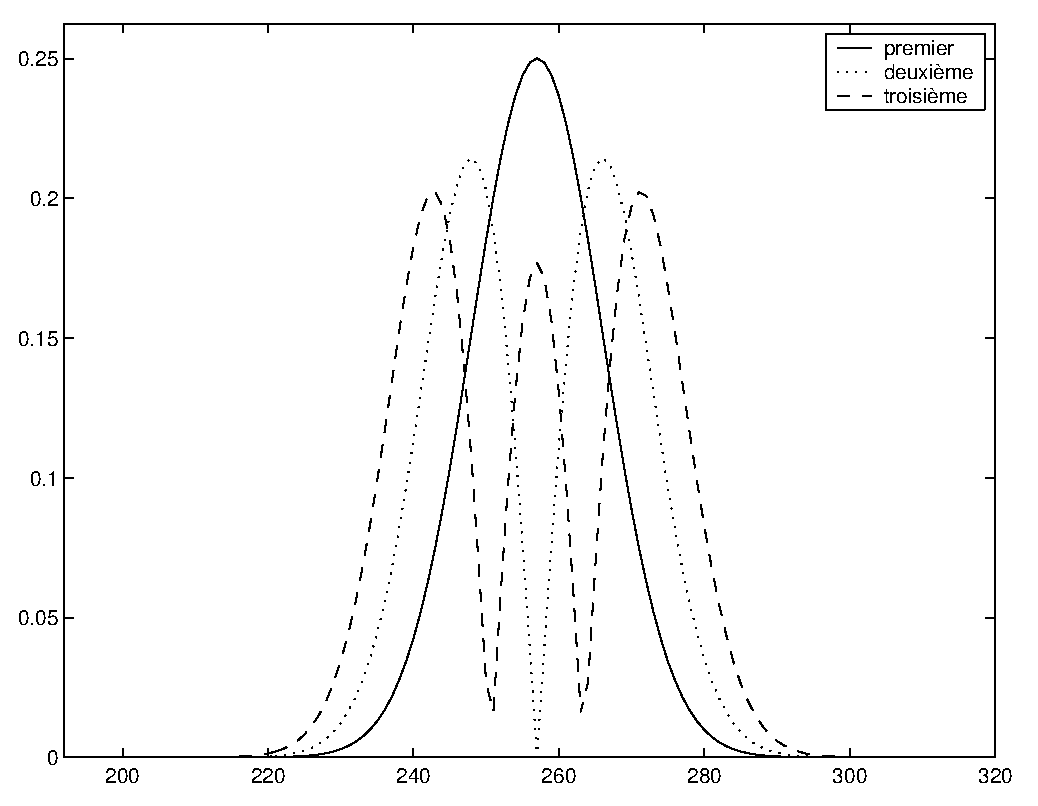
\includegraphics [scale = 0.4]{images/vecteurs-propres-tfd.eps}
    \end{center}
    \caption{Modules of some eigenvectors of $ \Omega_N $}
              \label{fig-eigenvectors-tfd}
\end{figure}
\begin{figure}[ht] 
    \begin{center}
    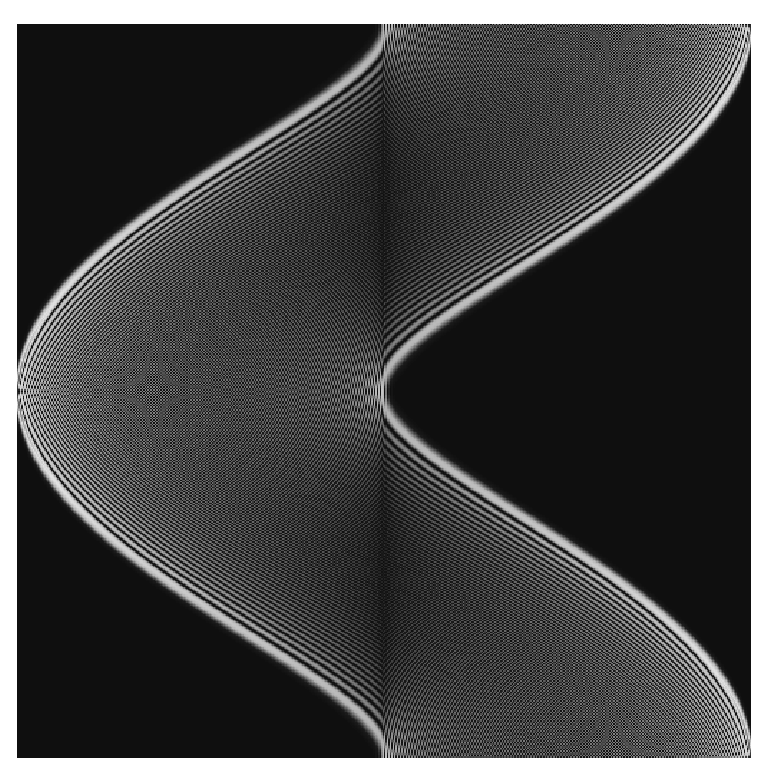
\includegraphics[scale=0.5]{images/matrice-vecteurs-propres-tfd.eps}
    \end{center}
    \caption{Matrix of moduli of orthogonal eigenvectors}
              \label{fig-matrix-eigenvectors-tfd}
\end{figure}
\end{exo}
 
 
\begin{exo}[Orthogonalization on a cyclic group]
\label{exo-orthogonalization-fourier}
 
This exercise studies in a particular case the notion of orthogonalization introduced in the exercise \oldref{exo-orthogonalization-abelian-group}. It is however independent. We consider the finite group $ G = \ZZ/n \ZZ $, as well as the vector space $ \CC [G] $ of functions from $ G $ in $ \CC $. For $ f \in \CC [G] $ and $ k \in G $, we define two actions of $ G $ on $ \CC [G] $ by setting
\begin{equation*}
k \top f: x \mapsto f(xk) \quad \quad \text{and} \quad \quad k \bot f: x \mapsto \omega^{- kx} f(x),
\end{equation*}
where we noted $ \omega_n \eqdef e^{\frac{2 \imath \pi}{n}} $. \begin{enumerate}
\item Show that the operations $ \top $ and $ \bot $ are related by
\begin{equation*}
\Ff(k \top f) = k \bot \Ff(f) \quad \quad \text{and} \quad \quad \Ff(k \bot f) = k \top \Ff(f).
\end{equation*}
 
\item We recall that $ f $ is said to be orthonormal under the action of $ \top $ if $ \{k \top f\}_{k \in G} $ is an orthonormal basis of $ \CC [G] $ . Using the previous question, explain how the orthonormal bases for $ \top $ and the orthonormal bases for $ \bot $ are related.
\item Show that $ f $ is orthonormal for $ \top $ if and only if $ \forall k \in G, \; | \wh{f}[k] | = $ 1.
\item Let $ f \in \CC [G] $ be such that $ \wh{f} $ does not vanish. We then define $ f_0 \in \CC [G] $ by
\begin{equation*}
\forall k \in G, \quad \wh{f_0}[k] = \frac{\wh{f}[k]}{| \wh{f}[k] |}.
\end{equation*}
Show that $ f_0 $ is orthonormal for $ \top $. Suggest a similar construction for $ \bot $.
\item \index{Correlation} We now assume that $ g $ is orthonormal for $ \top $. Let $ \varphi \in \CC [G] $ be any. We denote, for $ k \in G $, $ \Gg (\varphi) [k] \eqdef \dotp{\varphi}{k \top g} $ the decomposition coefficients of $ \varphi $ in the orthonormal basis $ \{k \top g\}_{k \in G} $. Show that $ \Gg (\varphi) = \frac{1}{n} f * \wt{g} \eqdef \frac{1}{n} \Corr (\varphi, \, g) $, where $ \wt{g}[k] \eqdef \ol{g [-k]} $, and $ \Corr $ is by definition the correlation of two vectors (see also the exercise \oldref{exo-correlation-2d} for the correlation of two images). Deduce a fast algorithm for calculating $ \Gg (\varphi) $ in $ O(n \log (n)) $ operations.
\end{enumerate} Figure \figref{fig-orthogonalisation-fourier} shows two examples of orthogonalization. The top function, which is closer to orthogonality than the bottom one (we see it on the moduli of Fourier coefficients which are far from $ 1 $), gives rise to a less oscillating function $ g $. Intuitively, to orthogonalize any function, we need the \guill{to oscillate}. \begin{figure}[ht]
    \begin{center}
    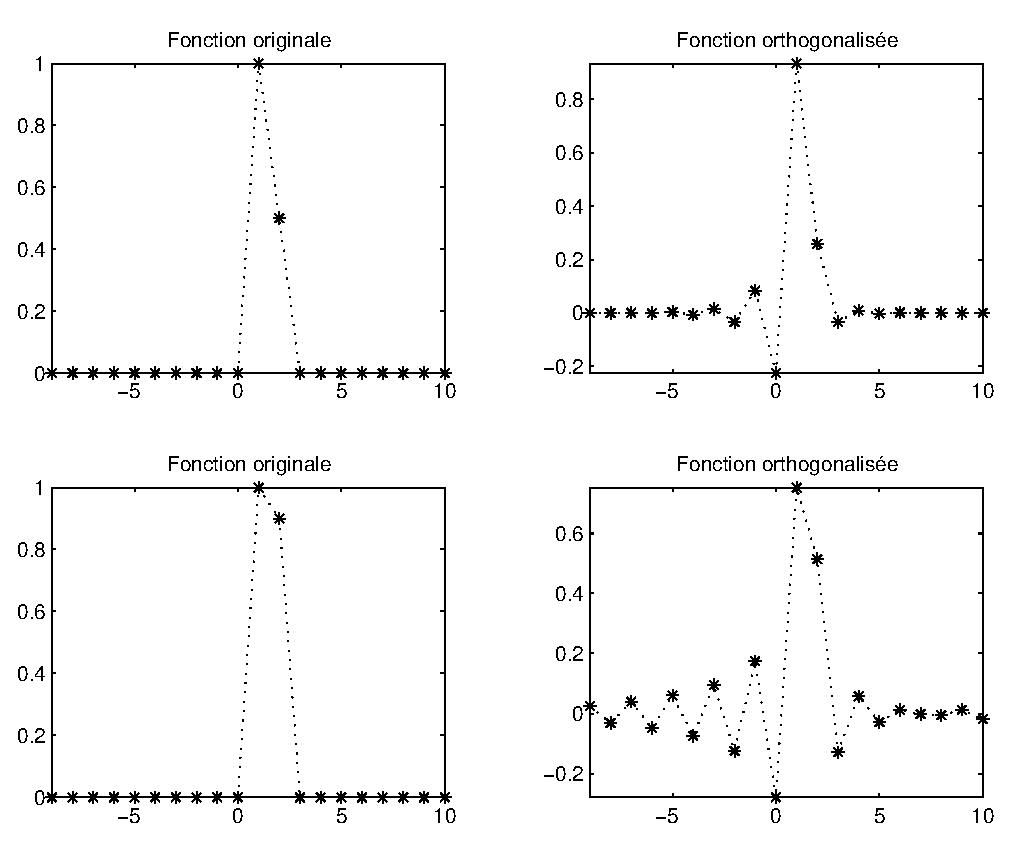
\includegraphics[scale=0.5]{images/orthogonalisation-fourier.eps}
    \end{center}
    \caption{Examples of orthogonalization}
              \label{fig-orthogonalisation-fourier}
\end{figure}
\end{exo}
 